%%% Template originaly created by Karol Kozioł (mail@karol-koziol.net) and modified for ShareLaTeX use

\documentclass[a4paper,10pt]{article}

\usepackage[
colorlinks=true,linkcolor=blue,urlcolor=blue,citecolor=blue,bookmarks=true,
bookmarksopenlevel=2]{hyperref}
\usepackage{amsmath,amssymb,amsthm,upgreek,textcomp,cancel,caption}
\usepackage{enumerate}
\usepackage{multicol}
\usepackage{tikz}
\usepackage{geometry}
\geometry{total={210mm,297mm},
left=25mm,right=25mm,%
bindingoffset=0mm, top=20mm,bottom=20mm}

\linespread{1.3}

\newcommand{\linia}{\rule{\linewidth}{0.5pt}}
% my own titles
\makeatletter
\renewcommand{\maketitle}{
\begin{center}
\vspace{2ex}
{\huge \textsc{\@title}}
\vspace{1ex}
\\
\linia\\
\@author
\vspace{4ex}
\end{center}
}
\makeatother
%%%

% custom footers and headers
\usepackage{fancyhdr,lastpage}
\pagestyle{fancy}
\lhead{}
\chead{}
\rhead{}
\renewcommand{\headrulewidth}{0pt}
\lfoot{Galactic Magnetism Study Guide}
\cfoot{}
\rfoot{Page \thepage\ /\ \pageref*{LastPage}}

%%%----------%%%----------%%%----------%%%----------%%%

\begin{document}
\hfill{\textit{Last modified \today}}
\title{Galactic Magnetism PhD Study Guide}
\author{Jessica Campbell, Dunlap Institute for Astronomy \& Astrophysics (UofT)}
\date{\today}
\maketitle
\tableofcontents

%%%%%%%%%%%%%%%%%%%%
%                                                          %
%                       PREFACE                  %
%                                                          %
%%%%%%%%%%%%%%%%%%%%

\section{Preface}

The interstellar medium (ISM) is a complex environment of gas and dust with varying degrees of ionization, densities, and spatial distributions called \textit{phases}. It accounts for $\sim10-15\%$ of the mass and $1-2\%$ of the volume of our Galaxy. From the largest of Galactic scales to the smallest scales of star and planet formation, this tenuous plasma is threaded with magnetic field lines and exhibits large degrees of turbulence, both of which are believed to be major driving forces in shaping the structure and dynamics of our Galaxy. These magnetic fields, along with cosmic rays, exert outward pressures on the ISM which are counterbalanced by the gravitational attraction provided by the ordinary matter. The ordinary matter, cosmic rays, and magnetic fields are therefore in a state of pressure equilibrium. Turbulence is an important aspect of the ISM as it not only transports energy from large ($\sim$kpc) to small ($\sim$pc) scales, but also amplifies magnetic fields and accelerates cosmic rays, explaining the observed $\mu$G magnetic field strengths as well as the $\sim$GeV cosmic ray energies in our Galaxy. Turbulence itself is a complex nonlinear fluid phenomenon which results in an extreme range of correlated spatial and temporal scales in the multi-phase ISM, and is driven by a variety of large- and small-scale energy sources. While magnetic fields and turbulence are generally understood to play fundamental roles in shaping the structure and dynamics of our Galaxy, the degree to which they do so across different phases and spatial scales of the ISM remains poorly understood. As such, this will be the focus of my thesis work!

































%%%%%%%%%%%%%%%%%%%%
%                                                          %
%                     TERMINOLOGY           %
%                                                          %
%%%%%%%%%%%%%%%%%%%%

\newpage
\section{Terminology}

{\noindent}\textbf{Advection:} The transport of a substance by bulk motion.

{\noindent}\textbf{Advection operator:}

{\noindent}\textbf{Alfv\'en Mach number:} A commonly used parameter of turbulence used to obtain information on gas compressibility and magnetization.

{\noindent}\textbf{Alfv\'en speed ($V_A$):} Given by

\begin{align*}
    V_A = \frac{B}{4\pi\rho_n} ~ [{\rm m\,s^{-1}}],
\end{align*}

{\noindent}where $B$ is the magnetic field strength and $\rho$ is the density of neutral particles. When the Alfv\'en speed is greater than the sound speed, the fast and Alfv\'en wave families are damped at or below the \textit{ambipolar diffusion scale} $L_\mathrm{AD}$; when the Alfv\'en speed is less than the sound speed, the slow and Alfv\'en wave families are damped.

{\noindent}\textbf{Alfv\'en wave:} A type of magnetohydrodynamic (MHD) wave in which ions oscillate in response to a restoring force provided by an effective tension on the magnetic field lines.

{\noindent}\textbf{Ambipolar diffusion:} The drift of neutral particles towards the central gravitational potential through the ionized particles tied to the magnetic field. This is often invoked as a source of dissipation of the magnetohydrodynamic (MHD) energy cascade. The scale at which ions and neutral particles decouple is called the \textit{ambipolar diffusion scale}. The application of ambipolar diffusion extends beyond direct studies of star formation and to include general studies of magnetic fields. Ambipolar diffusion has been proposed to damp particular families of MHD waves. 

{\noindent}\textbf{Ambipolar diffusion scale ($L_\mathrm{AD}$):} The scale at which ions and neutral particles decouple through the process of \textit{ambipolar diffusion}. It can be estimated as the scale at which the \textit{Reynolds number}, with diffusivity given by ambipolar diffusivity, is equal to unity. The ambipolar diffusion scale has been thought to set the dissipation scale of turbulence in molecular clouds and set a fundamental characteristic scale for gravitational collapse in star formation. When the Alfv\'en speed is greater than the sound speed, the fast and Alfv\'en wave families are damped at or below the \textit{ambipolar diffusion scale} $L_\mathrm{AD}$; when the Alfv\'en speed is less than the sound speed, the slow and Alfv\'en wave families are damped. On scales larger than $L_\mathrm{AD}$, it was also predicted that two-fluid turbulence (ion-neutral) acts like single-fluid MHD turbulence. The \textit{ambipolar diffusivity} is given by

\begin{align*}
    \nu_\mathrm{AD} = \frac{B^2}{4\pi\rho_i\rho_n\alpha} ~ [{\rm m^s\,s^{-1}}],
\end{align*}

{\noindent}where $\rho_i$ and $\rho_n$ are the density of the ions and neutrals, respectively, $B$ is the magnetic field strength, and $\alpha$ is the frictional coupling coefficient between the ions and neutrals. The \textit{Reynolds number} for ion-neutral drift is defined as

\begin{align*}
    R_\mathrm{AD} = \frac{LV}{\nu_\mathrm{AD}} ~ [{\rm dimensionless}],
\end{align*}

{\noindent}where $V$ is a characteristic velocity (e.g., for trans-Alfv\'enic turbulence it is the Alfv\'en speed, $V_A = \dfrac{B}{4\pi\rho_n}$) and $L=L_\mathrm{AD}$ when $R_\mathrm{AD}=1$. This gives the form of the ambipolar diffusion scale as often found in the literature:

\begin{align*}
    L_\mathrm{AD} = \frac{V_A}{\alpha\rho_i} ~ [{\rm m}].
\end{align*}

{\noindent}It has been shown that the plane-of-sky magnetic field can be estimated using the ambipolar diffusion length scale. 

{\noindent}\textbf{Autocorrelation:} The correlation of a signal with a delayed copy of itself as a function of delay. Informally, it is the similarity between observations as a function of the time lag between them. The autocorrelation of an observable $A$ with position $r$ and position increment $\delta r$ is given by

\begin{align*}
    C(\delta r) = \langle f(r)f(r+\delta r)\rangle ~ [{\rm dimensionless}].
\end{align*}

{\noindent}\textbf{Axi-symmetric spiral (ASS) model:}

{\noindent}\textbf{Balbus-Hawley instability:} Also known as the magnetorotational instability.

{\noindent}\textbf{Bandwidth depolarization:} A type of \textit{external depolarization} where the polarization vector is substantially rotated within the observing bandwidth if the Faraday depth is large enough.

{\noindent}\textbf{Beam depolarization:} A type of \textit{external depolarization} due to fluctuations in the foreground screen within the observing beam: unresolved density or magnetic field inhomogeneities of the media through which the radiation propagates induces unresolved spatial variations in the Faraday rotation measure.

{\noindent}\textbf{Birefringence:} The optical property of a medium to have a refractive index that is dependent on the polarization and direction of propagation of light. The magneto-ionic medium is an example of such a medium as the \textit{polarization angle} of light becomes rotated as it propagates via Faraday rotation as a function of frequency.

{\noindent}\textbf{Bi-symmetric spiral (BSS) model:}

{\noindent}\textbf{Bonnor-Ebert sphere:}

{\noindent}\textbf{Bremmstrahlung radiation:} Also known as "braking radiation". This radiation is produced by the deceleration of a charged particle after being deflected by another charged particle, typically an electron by an atomic nucleus. The particle being deflected loses energy which is lost via radiation of a photon. For example, when free electrons within an H$_\mathrm{II}$ region pass near a positive ion (H$^+$, He$^+$) they are accelerated by the Coulomb field and emit bremsstrahlung radiation. Bremsstrahlung emission is a source of polarized continuum radiation and is a type of free-free radiation.

{\noindent}\textbf{Cascade rate:}

{\noindent}\textbf{Chaotic system:}

{\noindent}\textbf{Coherent magnetic field:} Also known as an ordered magnetic field.

{\noindent}\textbf{Cold neutral medium (CNM):}

{\noindent}\textbf{Complex conjugate (${f(x)}^*\,{\rm or}\,\bar{f}(x)$):} The number with an equal real part and an imaginary part equal in magnitude but opposite in sign.

{\noindent}\textbf{Compressible turbulence:}

{\noindent}\textbf{Compton scattering:} The inelastic scattering of a photon by a free charged particle (usually an electron) in which energy is lost from the photon (typically a gamma ray or X-ray) which is in part transferred to recoiling the charged particle.

{\noindent}\textbf{Cosmic rays:} Extremely energetic and electrically charged particles pervading the ISM. The Galactic origin of the most energetic cosmic rays and their widespread distribution throughout the Milky Way was not recognized until the observed Galactic radio emission was correctly identified with \textit{synchrotron radiation} emitted by cosmic-ray electrons gyrating about the local Galactic magnetic field. Cosmic rays impinge on the ISM in three important ways: (1) they contribute to its ionization through direct collisions with gas particles, (2) they constitute a triple source of heating arising from the excess energy carried away by the electrons released in cosmic-ray ionization, from Coulomb encounters with charged particles of gas particles, and from the damping of Alfv\'en waves excited by cosmic rays streaming along magnetic field lines, and (3) they are dynamically coupled to the ISM via the magnetic field.

{\noindent}\textbf{Delta variance ($\sigma_\Delta^2(L)$):} A way to measure power on various scales defined as

\begin{align*}
    \sigma_\Delta^2(L) = \left\langle \int\limits_0^{3L/2} {(A[r+x]-\langle A\rangle)\odot(x)}^2\mathrm{d}x \right\rangle,
\end{align*}

{\noindent}for a two-step function

\begin{equation*}
\odot(x) = \pi\left(\frac{L}{2}\right)^{-2} \times
\left\{
\begin{aligned}
1,          ~~~~~& \mathrm{if}\,x<(L/2) \\
-0.125, ~~~~~& \mathrm{if}\,(L/2)x<(3L/2)
\end{aligned}
\right.
.
\end{equation*}

{\noindent}The delta variance is related to the \textit{power spectrum} $P(k)$: for an emission distribution with a power spectrum $P(k)\propto k^{-n}$ for wavenumber $k$, the delta variance is $\sigma_\Delta^2(L)\propto r^{n-2}$ for $r=1/k$.

{\noindent}\textbf{Depolarization:} A reduction in the degree of polarization, measured as the ratio of the observed to the intrinsic polarization, either at a given frequency or when comparing two frequencies. Such depolarization can be caused by Faraday rotation in two different circumstances: \textit{internal depolarization} or \textit{external depolarization}. In order to distinguish between internal and external depolarization, very high resolution and sensitive polarization data at multiple frequencies are needed. The key difference is that internal depolarization should be correlated with the Faraday RM (such that regions with small RM exhibit low amounts of depolarization) whereas external depolarization should be correlated with the gradient of the RM.

{\noindent}\textbf{Depolarization canals:} Caused either by resolution-element or line-of-sight effects.

{\noindent}\textbf{Depth depolarization:}

{\noindent}\textbf{Dispersion measure (DM):}

\begin{align*}
    {\rm DM} = -\int\limits_\mathrm{source}^\mathrm{observer} n_e\vec{{\rm d}\ell} ~ [{\rm pc\,cm^{-3}}]
\end{align*}

{\noindent}\textbf{Dust polarization:} The polarization angle of dust emission is conventionally taken to be $90^\circ$ from the orientation of the local Galactic magnetic field.

{\noindent}\textbf{Dynamo theory:} The mechanism by which a magnetic field is produced in which a rotating, convecting, and electrically conducting fluid can generate and maintain a magnetic field over astronomical timescales. 

{\noindent}\textbf{Eddies:}

{\noindent}\textbf{Eddy interaction rate:}

{\noindent}\textbf{Emission measure (EM):} The square of the number density of free electrons integrated over the volume of plasma.

\begin{align*}
    {\rm EM} = -\int\limits_\mathrm{source}^\mathrm{observer} n_e^2\vec{{\rm d}\ell} ~ [{\rm pc\,cm^{-6}}]
\end{align*}

{\noindent}\textbf{Energy cascade:}

{\noindent}\textbf{Energy spectrum ($E(k)$):} The term energy refers to any squared quantity, not necessarily velocity.

{\noindent}\textbf{Epicycles:} Small oscillations that Galactic disk stars experience about a perfectly circular orbit in the Galactic plane due to their velocity dispersion of $\sim10-40\,{\rm km\,s^{-1}}$ about their $\simeq220\,{\rm km\,s^{-1}}$ rotational velocity.

{\noindent}\textbf{External depolarization:} Depolarization induced by the limitations of the instrumental capabilities. For example, \textit{beamwidth depolarization} is due to fluctuations in the foreground screen within the observing beam: unresolved density or magnetic field inhomogeneities of the media through which the radiation propagates induces unresolved spatial variations in the Faraday rotation measure. Another form of external depolarization is \textit{bandwidth depolarization} which can occur when a signification rotation of the \textit{polarization angle} is produced across the observing bandwidth.

{\noindent}\textbf{Faraday depth $(\phi)$:} The Faraday depth of a source is defined as

\begin{align*}
    \phi(\mathbf{r}) = -0.81 \int\limits_\mathrm{source}^\mathrm{observer}n_e\vec{B}\cdot\vec{{\rm d}r} ~ [{\rm rad\,m^{-2}}],
\end{align*}

{\noindent}where $n_e$ is the electron density in ${\rm cm^{-3}}$, $\vec{B}$ is the magnetic field strength in $\mu{\rm G}$, and $\vec{{\rm d}r}$ is an infinitesimal path length in ${\rm pc}$. The negative sign sets the convention that $\phi$ is positive for a $B$ direction pointing towards the observer. Most compact sources like pulsars and extremely compact extragalactic sources show a single value of $\phi$, called the \textit{rotation measure} (RM). The Faraday depth (or RM) does not increase monotonically with distance along the line of sight.

{\noindent}\textbf{Faraday dispersion:} A type of \textit{internal depolarization} caused by emission at different Faraday depths along the same line of sight.

{\noindent}\textbf{Faraday dispersion function ($F(\phi)$):} Also referred to as the \textit{Faraday spectrum} introduced by Burn (1966) which describes the complex polarization vector as a function of Faraday depth as

\begin{align*}
    F(\phi) = \int\limits_{\infty}^\infty P(\lambda^2)\mathrm{e}^{-2i\phi\lambda^2}\mathrm{d}\lambda^2 ~ [{\rm rad\,m^{-2}}],
\end{align*}

{\noindent}where $F(\phi)$ is the complex polarized surface brightness per unit Faraday depth and $P(\lambda^2) = p(\lambda^2)I(\lambda^2)$ is the complex polarized surface brightness. To obtain the Faraday dispersion function, \textit{rotation measure (RM) synthesis} is used to Fourier transform the observed polarized surface brightness into the Faraday spectrum. This Faraday dispersion function is not straightforward to interpret; in particular, there is no direct relationship between Faraday depth and physical depth. Further, the Faraday dispersion function suffers from sidelobes of the main components caused by limited coverage of the observed wavelength space. Burn (1966) assumes that $F(\phi)$ is independent of frequency. The equation for $P(\lambda^2)$ is very similar to a Fourier transform; a fundamental difference is that $P(\lambda^2)$ only has physical meaning for $\lambda\geq0$. Since $P(\lambda^2)$ cannot be measured for $\lambda<0$, it is only invertible if one makes assumptions about the values of $P$ for $\lambda^2<0$ based on those for $\lambda^2\geq0$ (Burn 1966). For example, assuming that $P(\lambda^2)$ is Hermitian corresponds to assuming that $F(\phi)$ is strictly real.

{\noindent}\textbf{Faraday rotation:} A frequency-dependent magneto-optical phenomenon (i.e., an interaction between light and a magnetic field) in which the plane of polarization is rotated by an amount that is linearly proportional to the strength of the magnetic field in the direction of propagation. Faraday rotation results from the fact that right-handed circularly (RHC) and left-handed circularly (LHC) polarized light experience different phase velocities when traveling through a magneto-ionic medium. Faraday rotation is induced by thermal electrons (not synchrotron radiation) coincident with a magnetic field which is at least partially oriented along the line of sight between the source and the observer. The Faraday rotation is used to measure the parallel component of the magnetic field via ionized gas. Given an initial polarization angle $\chi_0$ and an observing frequency $\lambda^2$, the observed polarization angle is a function of the Faraday depth $\phi$ of the medium at a given physical distance $\mathbf{r}$ given by

\begin{align*}
    \chi = \chi_0 + \phi(\mathbf{r}) \lambda^2 ~[{\rm rad}].
\end{align*}

{\noindent}When a straight line is fit to this equation to provide a single value for $\phi(\mathbf{r})$, this is traditionally called the \textit{rotation measure} (RM). This would only be a valid approximation for the simplest of cases, for example, a single foreground medium inducing Faraday rotation that is itself not emitting its own polarized emission. In more complex scenarios, polarized synchrotron emission may originate from volumes that are also inducing Faraday rotation which leads to polarized synchrotron emission at a range of Faraday depths. In such situations, \textit{rotation measure synthesis} (RM-synthesis) must be done to obtain the Faraday depth as a function of physical distance, $\phi(\mathbf{r})$. The Faraday depth $\phi(\mathbf{r})$ is a proportionality constant that encapsulates the physics of the situation:

\begin{align*}
    \phi(\mathbf{r}) = -0.81 \int\limits_\mathrm{source}^\mathrm{observer}n_e\vec{B}\cdot\vec{{\rm }r} ~ [{\rm rad\,m^{-2}}].
\end{align*}

{\noindent}Additional complications may arise if the Faraday depth is large enough to substantially rotate the polarization vector within the observing bandwidth, an effect known as \textit{bandwidth depolarization}.

{\noindent}\textbf{Faraday spectrum:} See \textit{Faraday dispersion function}.

{\noindent}\textbf{Faraday screen:} A background emitting source of radiation which experiences Faraday rotation by a foreground source. In this case,  and Faraday depth are identical; otherwise Rotation Measure Synthesis is needed.

{\noindent}\textbf{Faraday thick:} A source is Faraday thick if the wavelength squared times the extent of the object in units of Faraday depth is much greater than 1: $\lambda^2\Delta\phi\gg1$. In the case of Faraday thick, objects are extended in Faraday space and substantially depolarized at wavelength squared. Remember that whether an object is Faraday thin or Faraday thick is wavelength dependent.

{\noindent}\textbf{Faraday thin:} A source is Faraday thin if the wavelength squared times the extent of the object in units of Faraday depth is much less than 1: $\lambda^2\Delta\phi\ll1$. In the case of Faraday thin, objects are well approximated by a Dirac-delta function in Faraday space. Remember that whether an object is Faraday thin or Faraday thick is wavelength dependent.

{\noindent}\textbf{Filling factor:} See \textit{volume filling factor}.

{\noindent}\textbf{Fluid turbulence:}

{\noindent}\textbf{Flux freezing:} The coupling between the \textit{cold neutral medium} (CNM) and the magnetic field due to its non-zero ionization fraction.

{\noindent}\textbf{Forbidden line:} Also known as a \textit{forbidden mechanism} or a \textit{forbidden transition}. A spectral line associated with the emission or absorption of light by atomic nuclei, atoms, or molecules which undergo a transition that is not allowed by a particular selection rule but does occur if the approximation associated with that rule is not made. Forbidden emission lines have been observed in extremely low-density gas and plasma in which collisions are infrequent. Under such conditions, once an atom or molecule has been excited for any reason into a meta-stable state, it is almost certain to decay by emission of a forbidden-line photon. Since meta-stable states are rather common, forbidden transitions account for a significant percentage of the photons emitted by the ultra-low density gas in space.

{\noindent}\textbf{Fourier transform ($\hat{f}(x)$):} Decomposes a function of time (a signal) into the frequencies that make it up. The Fourier transform (FT) of a function $f(x)$ is given by

\begin{align*}
    \hat{f}(x) = \int\limits_{-\infty}^\infty f(x')e^{-2\pi ixx'}dx'.
\end{align*}

{\noindent}The reason for the negative sign convention in the definition of $\hat{f}(x)$ is that the integral produces the amplitude and phase of the function $f(x')e^{-2\pi xx'}$ at frequency zero ($0$), which is identical to the amplitude and phase of the function $f(x')$ at frequency $x'$ , which is what $\hat{f}(x)$ is supposed to represent. The function $f(x)$ can be reconstructed from its Fourier transform $\hat{f}(x)$, which is known as the Fourier inverse theorem.

{\noindent}\textbf{First moment:} 

{\noindent}\textbf{Fractional polarization $(p(\alpha))$:}

{\noindent}\textbf{Great circle:} A circle on the surface of a sphere that lies in a plane passing through the sphere's center which represents the shortest distance between any two points on the surface of a sphere.

{\noindent}\textbf{Gyration frequency ($\omega$):} The angular frequency of circular motion.

{\noindent}\textbf{Hot ionized medium (HIM):} Diffuse interstellar gas with a typical temperature of $T\sim10^5-10^6\,{\rm K}$. This hot interstellar gas is believed to have been generated mainly by \textit{supernovae} and stellar winds from massive stars, forming as the shock wave sweeps through the \textit{interstellar medium}.

{\noindent}\textbf{Hydrogen spectral series:} Six named Hydrogen line series describing the emission spectrum of Hydrogen as dictated by the Rydberg equation. Includes the Lyman series ($n'=1$), Balmer series ($n'=2$), Paschen (or Bohr) series ($n'=3$), Brackett series ($n'=4$), Pfund series ($n'=5$), Humphreys series ($n'=6$).

{\noindent}\textbf{H$_\mathrm{II}$ region:} The ionized clouds around massive OB stars which are responsible for ionizing most of the hydrogen around such stars. The boundaries of H$_\mathrm{II}$ regions are determined by the volume in which the rate of UV photoionization equals the rate of recombination of electrons. When free electrons within an H$_\mathrm{II}$ region pass near a positive ion (H$^+$, He$^+$) they are accelerated by the Coulomb field and emit radiation known as ``free-free'' or \textit{bremsstrahlung emission} which is a source of polarized continuum emission. The average electron density of an H$_\mathrm{II}$ region is $\sim10^3\,{\rm cm^{-3}}$.

{\noindent}\textbf{Incompressible turbulence:} The \textit{Kolmogorov power spectrum} for incompressible turbulence in three dimensions is $P(k)\propto k^{-11/3}$ while its \textit{energy spectrum} is $E(k)\propto k^{-5/3}$. In two dimensions, $P(k)\propto k^{-8/3}$ and $E(k)\propto k^{-5/3}$ (unchanged). For one dimension, $P(k)\propto k^{-5/3}$ and $E(k)\propto k^{-5/3}$ (unchanged).

{\noindent}\textbf{Infrared polarization:} The same large-scale alignment of aspherical, spinning dust grains that causes \textit{starlight polarization} also causes polarization of far-infrared emission.

{\noindent}\textbf{Internal depolarization:} Depolarization due to the spatial extent of the source and occurs even if the intervening media are completely homogenous. Along the line of sight, the emission from individual electrons within a source arrive from different depths and suffer different Faraday rotation angles due to different path lengths. For the total radiation emitted by a source, this results in a reduction of the observed degree of polarization.

{\noindent}\textbf{Interstellar medium (ISM):} A tenuous medium throughout galaxies that consists of three basic constituents: (1) ordinary matter, (2) relativistic charged particles called cosmic rays, and (3) magnetic fields. These three basic constituents have comparable pressures and are bound together by electromagnetic forces. The ordinary matter itself consists of gas (atoms, molecules, ions, and electrons) and dust (tiny solid particles) which can exist in a number of phases: molecular, cold atomic, warm atomic, warm ionized, and hot ionized. Apart from the densest parts of molecular clouds whose degree of ionization is exceedingly low, virtually all interstellar regions are sufficiently ionized for their neutral component to remain tightly coupled to the charged component and hence to the local magnetic field. Cosmic rays and magnetic fields influence both the dynamics of the ordinary matter and its spatial distribution at all scales, providing, in particular, an efficient support mechanism against gravity. Conversely, the weight of the ordinary (i.e., baryonic) matter confines magnetic fields and, hence, cosmic rays to the Galaxy, while its turbulent motion can be held responsible for the amplification of magnetic fields and for the acceleration of cosmic rays. Studies of the diffuse ($n\sim0.1-100\,{\rm cm^{-3}}$) HI suggests that the magnetic field strength is relatively independent of its volume density, in contrast to magnetic fields in molecular clouds. The Galactic origin of the most energetic cosmic rays and their widespread distribution throughout the Milky Way was not recognized until the observed Galactic radio emission was correctly identified with \textit{synchrotron radiation} emitted by cosmic-ray electrons gyrating about the local Galactic magnetic field. The ISM encloses but a small fraction of the total mass of the Galaxy. Moreover, it does not shine in the sky as visibly as stars do, yet it plays a vital role in many of the physical and chemical processes taking place in the Galactic ecosystem. The ISM is not merely a passive substrate within which stars evolve; it constitutes their direct partner in the Galactic ecosystem, continually exchanging matter and energy with them and controlling many of their properties. It is the spatial distribution of the ISM together with its thermal and chemical characteristics that determines where new stars form as well as their mass and luminosity spectra. These in turn govern the overall structure, optical appearance, and large-scale dynamics of our Galaxy. Hence understanding the present-day properties of our Galaxy and being able to predict its long-term evolution requires a good knowledge of the dynamics, energetics, and chemistry of the ISM. Table \ref{table:ismphases} outlines the different phases of the interstellar gas, including their typical temperature, number density, mass density, and total mass.

\begin{table}[h]
\begin{center}
\captionof{table}{Descriptive parameters of the different components of the interstellar gas. $T$ is the temperature, $n$ is the true (as opposed to space-averaged) number density of hydrogen nuclei near the Sun, $\Sigma_\odot$ is the azimuthally averaged mass density per unit area at the solar circle, and $\mathcal{M}$ is the mass contained in the entire Milky Way. Both $\Sigma_\odot$ and $\mathcal{M}$ include 70.4\% hydrogen, 28.1\% helium, and 1.5\% heavier elements. All values were rescaled to $R_\odot=8.5\,{\rm kpc}$ Table taken from Ferri\'ere (2001).} \label{table:ismphases}
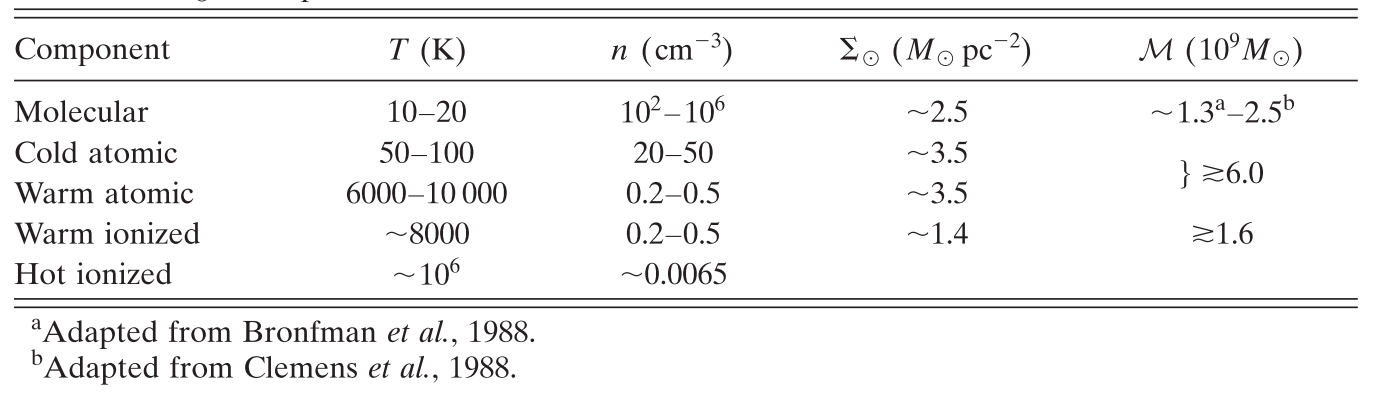
\includegraphics[width=15cm]{figures/ISMphases.png}
\end{center}
\end{table}

{\noindent}\textbf{Inverse Compton scattering:} The upscattering of radio photons to become optical or X-ray photons by means of the inelastic scattering of a charged particle (usually an electron).

{\noindent}\textbf{Inverse Fourier transform (IFT):} The reconstruction of a function from its decomposition into the frequencies that make it up. The inverse Fourier transform (IFT) is given by

\begin{align*}
    f(x) = \int\limits_{-\infty}^\infty \hat{f}(x')e^{2\pi ixx'}dx'.
\end{align*}

{\noindent}The fact that a function $f(x)$ can be reconstructed from its Fourier transform $\hat{f}(x)$ is known as the Fourier inverse theorem.

{\noindent}\textbf{Kelvin-Helmholtz instability:}

{\noindent}\textbf{Kolmogorov microscale:}

{\noindent}\textbf{Kolmogorov spectrum:}

%{\noindent}\textbf{Kolmogorov ction:}

{\noindent}\textbf{Kurtosis:}

{\noindent}\textbf{Lorentz factor ($\gamma$):} The factor by which time, length, and relativistic mass change for an object while that object is moving with speed $\mathbf{v}$:

\begin{align*}
    \gamma = \sqrt{\frac{1-(v/c)^2}{c^2}}.
\end{align*}

{\noindent}For non-relativistic motion $\gamma\approx1$, while for relativistic motion $\gamma>1$. For example, $\gamma(v=0.9c)\approx2$ and $\gamma(v=0.99c)\approx7$.

{\noindent}\textbf{Lorentz force:} The combination of electric and magnetic force on a point charge due to electromagnetic fields. A particle of mass $m$ and charge $q$ moving with a velocity $v$ within a magnetic field $\mathbf{B}$ experiences a force 

\begin{align*}
    F = \dfrac{\mathrm{d}}{\mathrm{d}\tau} (m\gamma\mathbf{v}) = q\left(\dfrac{\mathbf{v}}{c}\times\mathbf{B}\right) ~ [{\rm N}],
\end{align*}

{\noindent}where $\tau$ is the retarded time and $\gamma$ is the Lorentz factor. Of course, the Lorentz force only acts on charged particles but its effect is then transmitted to neutral particles via ion-neutral collisions.

{\noindent}\textbf{Mach number:}

{\noindent}\textbf{Magnetic buoyancy:} See Rayleigh-Taylor instability.

{\noindent}\textbf{Magnetic reconnection:}

{\noindent}\textbf{Magnetoionic medium (MIM):}

{\noindent}\textbf{Magnetorotational instability:} See Balbus-Hawley instability.

{\noindent}\textbf{Meridian:} A circle of constant longitude passing through a given place on Earth's surface and the terrestrial poles.

{\noindent}\textbf{Microturbulence:}

{\noindent}\textbf{Milky Way Galaxy (MWG):} We see the Milky Way as a narrow band encircling us because the Galaxy has the shape of a flattened disk within which we are deeply embedded. Our Galaxy comprises a thin disk with radius $\sim25-30\,{\rm kpc}$ and effective thickness $\sim400-600\,{\rm pc}$, plus a spherical system itself composed of a bulge with radius $\sim2-3\,{\rm kpc}$ and a halo extending out to more than $30\,{\rm kpc}$ from the center. The Sun resides in the Galactic disk, approximately $15\,{\rm pc}$ from the midplane and $8.5\,{\rm kpc}$ away from the center. The stars belonging to the disk rotate around the Galactic center in nearly circular orbits. Their angular rotation rate is a decreasing function of their radial distance. At the Sun's orbital distance, the Galactic rotation velocity is $\simeq220\,{\rm km\,s^{-1}}$, corresponding to a rotational period of $\simeq240\times10^6\,{\rm years}$. Disk stars also have a velocity dispersion of $\sim10-40\,{\rm km\,s^{-1}}$ which causes them to experience small oscillations about a perfectly circular orbit both in the Galactic plane (epicycles) and the vertical direction. In contrast, stars in the bulge and the halo rotate slowly and often have very eccentric orbits. Radio observations of interstellar neutral hydrogen indicate that the Milky Way possesses a spiral structure similar to those seen in optical wavelengths of external galaxies. The exact spiral structure of our own Galaxy is difficult to determine from within; the best radio data to date points to a structure characterized by a bulge of intermediate size and a moderate winding of the spiral arms. Infrared (IR) images of the Galactic center clearly display the distinctive signature of a bar. Our position in the spiral pattern can be derived from local optical measurements which give quite an accurate outline of the three closest arms; they locate the Sun between the inner Sagittarius arm and the outer Perseus arm, near the inner edge of the local Orion-Cygnus arm.

{\noindent}\textbf{$\mathbf{n\pi}$ ambiguity:} The inability to distinguish between polarization angles modulo $\pi$ radians, rendering traditional linear RM fits often arbitrary. One way to deal with this ambiguity is to rely on resolving smooth spatial gradients in the polarization angle at each wavelength. With this assumption, the appropriate value of $n$ can be resolved for each spatial pixel, yielding the correct polarization angle at each wavelength and thus the true value of RM. This is the basis of the PACERMAN routine developed by Dolag et al., (2005). However, routines like PACERMAN cannot deal with the second and third problems listed above since it is ultimately based on fitting a single value of RM along each line of sight. 

{\noindent}\textbf{Open cluster:} A rather loose, irregular grouping of $10^2-10^3$ stars confined to the Galactic disk and therefore also known as Galactic clusters. 

{\noindent}\textbf{Ordered magnetic field:} See coherent magnetic field.

{\noindent}\textbf{Paramagnetism:} Paramagnetic materials have unpaired electrons which, when in the presence of an external magnetic field such as the interstellar magnetic field, align in the same direction causing grain alignment.

{\noindent}\textbf{Parker instability:}

{\noindent}\textbf{Passive mixing:}

{\noindent}\textbf{Pitch angle:} The angle between a charged particle's velocity vector and the local magnetic field.

{\noindent}\textbf{Photodissociation region (PDR):} Also known as \textit{photon-dominated regions} or PDRs. Predominantly neutral regions of the ISM in which UV photons strongly influence the gas chemistry and act as the dominant energy source. They occur in any region of interstellar gas that is dense and cold enough to remain neutral, but that has too low of a column density to prevent penetration of far-UV photons from massive stars. They are also associated with HII regions. All of the atomic gas and most of the molecular gas is found in photodissociation regions.

{\noindent}\textbf{Photon-dominated region (PDR):} See \textit{photodissociation region}.

{\noindent}\textbf{Pitch angle:} The angle between a charged particle's velocity vector and the local magnetic field.

{\noindent}\textbf{Plasma beta ($\beta$):} The ratio of the gas to magnetic pressure. For either high or low $\beta$, it was predicted that \textit{Alfv\'en waves} should should damp at the \textit{ambipolar diffusion scale} $L_\mathrm{AD}$ and thus the magnetohydrodynamic (MHD) cascade should damp past the ambipolar diffusion scale.

{\noindent}\textbf{Poincaré sphere:}

{\noindent}\textbf{Polarized intensity ($P$):} A measure of the total linear polarization in radio emission given as

\begin{align*}
    P\equiv\sqrt{Q^2+U^2} ~ [{\rm Jy}],
\end{align*}

{\noindent}where $Q$ is the \textit{Stokes Q} polarization and $U$ the \textit{Stokes U} polarization. The images of $P$ (as well as $Q$ and $U$) are often filled with complex structures that bear little resemblance to the \textit{Stokes I} image of total intensity. The intensity variations seen in $P$ (as well as $Q$ and $U$) are the result of small-scale angular structure in the \textit{Faraday rotation} induced by ionized gas, and are thus an indirect representation of turbulent fluctuations in the free-electron density and magnetic field throughout the \textit{interstellar medium}. while $Q$ and $U$ exhibit Gaussian noise properties, this is not true for $P$. The noise in $Q$ and $U$ is squared when calculating $P$, having a Ricean distribution, and this causes the observed polarization intensity to be biased toward larger values

{\noindent}\textbf{Polarization angle $(\chi)$:} Given by

\begin{align*}
    \chi\equiv\frac{1}{2}\arctan\left(\frac{U}{Q}\right) ~ [{\rm rad}],
\end{align*}

{\noindent}where $Q$ is the \textit{Stokes Q} polarization vector and $U$ the \textit{Stokes U} polarization vector. The arctan2 function is generally used to determine $\chi$ over the full $\pm n\pi$ range. The polarization angle (likewise with the amplitude of \textit{polarized intensity}) is not preserved under arbitrary rotations and translations of the \textit{Q-U plane}. In the most general case, then, the observed values of $\chi$ (and $\mathbf{P}\equiv\sqrt{Q^2+U^2}$) do not have any physical significance; only measurements of quantities that are both rotationally and translationally invariant in the $Q-U$ plane can provide insight into the physical conditions that produce the observed polarization distribution.

{\noindent}\textbf{Polarization fraction $(p(\lambda^2))$:}

\begin{align*}
    p(\lambda^2) = \frac{P(\lambda^2)}{I(\lambda^2)} ~ [{\rm dimensionless}],
\end{align*}

{\noindent}where $P(\lambda^2)$ is the polarized surface brightness and $I(\lambda^2)$ is the total surface brightness.

{\noindent}\textbf{Polarization gradient ($\lvert\nabla \mathbf{P}\rvert$):} The rate at which the \textit{polarized intensity} complex vector $\mathbf{P}\equiv\sqrt{Q^2+U^2}$ traces out a trajectory in the \textit{Q-U} plane as a function of position on the sky given by

\begin{align*}
    \lvert\nabla P\rvert = \sqrt{\left(\frac{\partial Q}{\partial x}\right)^2 + \left(\frac{\partial U}{\partial x}\right)^2 + \left(\frac{\partial Q}{\partial y}\right)^2 + \left(\frac{\partial U}{\partial y}\right)^2} ~ [{\rm Jy\,beam^{-1}}],
\end{align*}

{\noindent}where $Q$ and $U$ are the complex \textit{Stokes vectors} and $x$ and $y$ are the Cartesian axes of the image plane. Note that $\lvert\nabla \mathbf{P}\rvert$ cannot be constructed from the scalar quantity $P\equiv\sqrt{Q^2+U^2}$, but is derived from the vector field $\mathbf{P}\equiv(Q,U)$. The amplitude of the polarization gradient $\lvert\nabla \mathbf{P}\rvert$ provides an image of magnetized turbulence in diffuse, ionized gas manifested as a complex filamentary web of discontinuities in gas density and magnetic field strength. This quantity is rotationally and translationally invariant in the $Q-U$ plane, and so has the potential to reveal properties of the polarized distribution that might otherwise be hidden by excess foreground emission or \textit{Faraday rotation}, or in data sets from which large-scale structure is missing. The polarization gradient is shown in Figure \ref{figure:delP}.

\begin{figure}[h]
\begin{center}
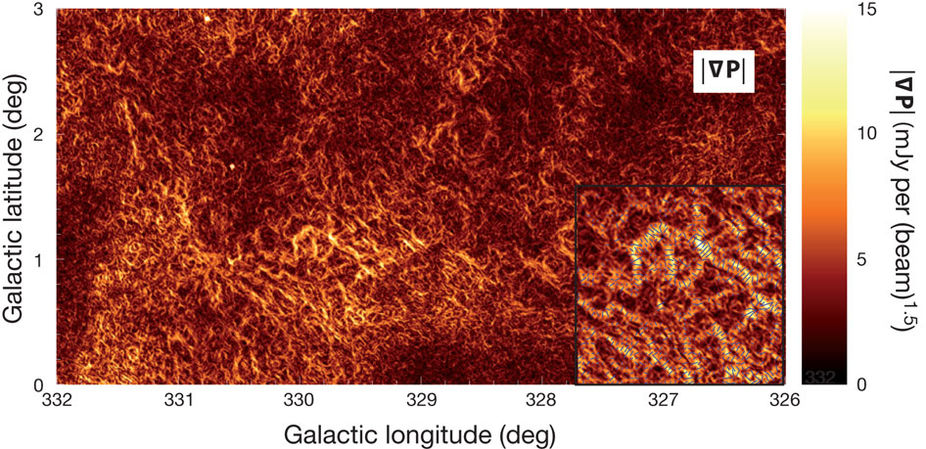
\includegraphics[width=15cm]{figures/delP.jpg}
\caption{$\lvert\nabla P\rvert$ for an $18$-deg$^2$ region of the Southern Galactic Plane Survey which reveals a complex network of tangled filaments. In particular, all regions in which $\lvert\nabla \mathbf{P}\rvert$ is high consists of elongated, narrow structures rather than extended patches. In the inset, the direction of $\lvert\nabla\mathbf{P}\rvert$ is shown for a small subregion of the image, demonstrating that $\lvert\nabla\mathbf{P}\rvert$ changes most rapidly along directions oriented perpendicular to the filaments. Figure taken from Gaensler (2011).}
\label{figure:delP}
\end{center}
\end{figure}

{\noindent}\textbf{Polarization gradient direction $(\mathrm{arg}\nabla \mathbf{P})$:} The direction of the \textit{polarization gradient} at a given spatial position defined as

\begin{align*}
    \mathrm{arg}(\nabla\mathbf{P}) \equiv \arctan \left[ \mathrm{sign} \left(\dfrac{\partial Q}{\partial x}\dfrac{\partial Q}{\partial y} + \dfrac{\partial U}{\partial x}\dfrac{\partial U}{\partial y}\right) \dfrac{\sqrt{\left(\dfrac{\partial Q}{\partial y}\right)^2 + \left(\dfrac{\partial U}{\partial y}\right)^2}}{\sqrt{\left(\dfrac{\partial Q}{\partial x}\right)^2 + \left(\dfrac{\partial U}{\partial x}\right)^2}} \right] ~ [{\rm rad}],
\end{align*}

{\noindent}where $Q$ and $U$ are the complex \textit{Stokes vectors}.

{\noindent}\textbf{Polarization horizon:} The furthest distance we can see diffuse polarized emission.

{\noindent}\textbf{Polarized surface brightness ($P(\lambda^2)$):} 

\begin{align*}
    P(\lambda^2) = p(\lambda^2)I(\lambda^2) = Q + iU ~ [{\rm Jy}],
\end{align*}

{\noindent}where $p(\lambda^2)$ is the polarization fraction, $I(\lambda)$ is the total surface brightness, and $Q$ and $U$ are the complex Stokes vectors. The absolute value of this complex vector is given by

\begin{align*}
    \lvert\lvert P(\lambda^2) \rvert\rvert = \sqrt{Q^2 + U^2} ~ [{\rm Jy}],
\end{align*}

{\noindent}where $Q$ and $U$ are the complex Stokes vectors.

{\noindent}\textbf{Power spectrum ($P(k)$):} Describes the distribution of power into frequency components composing that signal defined as

\begin{align*}
    P(k) = \hat{f}(k){\hat{f}(k)}^*,
\end{align*}

{\noindent}for wavenumber $k$ where $\hat{f}(k)$ denotes the \textit{Fourier transform} (FT) and ${\hat{f}(k)}$ its \textit{complex conjugate}. The power spectrum is the \textit{Fourier transform} (FT) of the \textit{autocorrelation function}.

{\noindent}\textbf{Prandtl number:}

{\noindent}\textbf{$Q-U$ plane:} Translations and rotations within the $Q-U$ plane can result from one or more of a smooth distribution of intervening polarized emission, a uniform screen of foreground \textit{Faraday rotation}, and the effects of missing large-scale structure in an interferometric data set.

{\noindent}\textbf{Radial component of polarization gradient:}

\begin{align*}
    \frac{\partial\mathbf{P}}{\partial s}_\mathrm{rad} = \sqrt{\frac{(Q\frac{\partial Q}{\partial x} + U\frac{\partial U}{\partial x})^2 + (Q\frac{\partial Q}{\partial y} + U\frac{\partial U}{\partial y})^2}{Q^2+U^2}} ~ [{\rm Jy\,pc^{-1}}]
\end{align*}

{\noindent}\textbf{Random magnetic field:} See turbulent magnetic field.

{\noindent}\textbf{Rayleigh-Taylor instability:} Also known as magnetic buoyancy.

{\noindent}\textbf{Reynold's number:}

{\noindent}\textbf{Rolling Hough Transform (RHT):} A machine vision algorithm designed for detecting and paramaterizing linear structure in astronomical data, originally applied to HI images. The detection of astronomical linear structure is approached in various ways depending on the context. Because HI structures are not objects with distinct boundaries, the problem is fundamentally different from many others. As these diffuse HI fibers were not formed by gravitational forces, there is no reason to require that they must be, or bridge, local overdensities. Indeed, these fibers are found often to be in groups of parallel structures, very unlike the cosmic web. Thus, methods developed for gravitationally dominated systems are not optimal for these purposes. The RHT is, as its name suggests, a modification of the Hough transform. The Hough transform was first introduced in in a patent for the detection of complex patterns in bubble chamber photographs. It was soon recognized as a powerful line detection technique, and has found wide applications in image processing and machine vision. The adaption of the Hough transform with the RHT is a rolling version that is particularly well suited to the detection and quantization of specific linear features in astronomical data. The RHT does not merely identify fibers; it encodes the probability that any given image pixel is part of a coherent linear structure. This allows the user to quantify the linearity of regions of sky without specifying fibers as discrete entities. The RHT operates on two-dimensional data and is designed to be sensitive to linear structure irrespective of the overall brightness of the region. The first step is to unsharp mask the image. The image is convolved with a two-dimensional top-hat smoothing kernel of a user-defined diameter, $D_K$. The smoothed data is then subtracted from the original data  and the resulting map is thresholded at 0 to obtain a bitmask. The subtraction of the smoothed component can be considered a suppression of large-scale structure, or a high-pass Fourier filter. Each straight line is parameterized in terms of the angle $\theta$ of its normal, and its minimum Euclidean distance from the origin $\rho$,

\begin{align*}
    \rho = x\cos\theta+y\sin\theta ~ [{\rm pixels}].
\end{align*}

{\noindent}Every possible line in the image space is uniquely specified by a point in the $\rho-\theta$ space. The RHT mapping is performed on a circular domain, diameter $D_W$, centered on each image-space pixel $(x_0,y_0)$ in turn. Then a Hough transform is performed on this area, limited to $\rho=0$. Thus the $\rho-\theta$ space is reduced to a one-dimensional space on $\theta$ for each pixel. All intensity over a set intensity threshold $Z$ is stored as $R(\theta,x_0,y_0)$: RHT intensity as a function of $\theta$ for that pixel. $Z$ is a percentage. In every direction $\theta$, $Z\times D_W$ pixels must contain signal in order for the transform to record the data in that direction. We use the canonical binning for the number of theta bins:

\begin{align*}
    n_\theta = \left[\pi\frac{\sqrt{2}}{2}(D_W-1)\right] ~ [{\rm dimensionless}].
\end{align*}

{\noindent}By iterating (``rolling'') over the entire image space we produce the RHT output, $R(\theta,x,y)$. A visualization of the linear structures identified by the RHT, the \textbf{backprojection $R(x,y)$}, is obtained by integrating $R(\theta,x,y)$ over $\theta$:

\begin{align*}
    R(x,y) = \int R(\theta,x,y)\mathrm{d}\theta ~ [{\rm dimensionless}].
\end{align*}

{\noindent}One advantage of the RHT is that the input parameters of the transform can be chosen to highlight specific linear features of interest. One defines, for a given run of the RHT, a smoothing kernel diameter ($D_K$), a window diameter ($D_W$), and an intensity threshold ($Z$). The rolling nature of the RHT ensures that linear structure at least as long as $D_W$ will be identified. Thus $D_W$, along with the $Z$, sets a lower limit for the spatial length of the linear features. Thresholding below 100\% ($Z<1$) reflects the fact that structures can be physically coherent even if they are not visibly connected. $R(\theta,x,y)$ is intensity as a function of angle on a domain $\theta\in[0,\pi)$, as a $0^\circ$ orientation is equivalent to a $180^\circ$ orientation. $R(\theta,x,y)$ can be sampled in a circular region around each star in the field as

\begin{align*}
    R_*(x,y) = \int\int_\mathrm{disk} R(\theta,x,y)\mathrm{d}x\mathrm{d}y ~ [{\rm dimensionless}].
\end{align*}

{\noindent}To estimate the direction of a given region of the backrprojection $R_*(\theta,x,y)$, the expectation value is given by

\begin{align*}
    \langle\theta\rangle' = \frac{1}{2}\arctan \left[\frac{\int\sin(2\theta)R_*(\theta)\mathrm{d}\theta}{\int\cos(2\theta)R_*(\theta)\mathrm{d}\theta}\right] ~ [{\rm rad}]
\end{align*}

{\noindent}where the equivalent value is found on the interval $\theta\in[0,\pi)$ via

\begin{align*}
    \langle\theta\rangle = \pi - {\rm mod}(\langle\theta\rangle'+\pi,\pi) ~ [{\rm rad}].
\end{align*}

{\noindent}Linear polarization data can be fully described by either
a polarization angle $\chi$ and polarized intensity $P$ or by the Stokes parameters $Q$ and $U$, where $\chi=(1/2)\arctan(U/Q)$ and $P=\sqrt{Q^2+U^2}$. From the RHT output, similar `Stokes vectors' can be defined via

\begin{align*}
    Q_\mathrm{RHT} = \int\cos(2\theta)R(\theta)\mathrm{d}\theta ~ [{\rm Jy}] \\
    U_\mathrm{RHT} = \int\sin(2\theta)R(\theta)\mathrm{d}\theta ~ [{\rm Jy}].
\end{align*}

{\noindent}This allows for an estimate of the orientation of the magnetic field to be derived solely from HI data via

\begin{align*}
    \theta_\mathrm{RHT} = \frac{1}{2}\arctan\left(\frac{U_\mathrm{RHT}}{Q_\mathrm{RHT}}\right) ~ [{\rm rad}].
\end{align*}

{\noindent}\textbf{Rotation measure (RM):} Characterizes the amount of \textit{Faraday rotation} that polarized light experiences while passing through thermal electrons. Most compact polarized sources like pulsars and extremely compact extragalactic sources show a single value of Faraday rotation which is the RM. This is commonly defined as the slope of the polarization angle $\chi$ versus $\lambda^2$ plot:

\begin{align*}
    {\rm RM} = \frac{\mathrm{d}\chi(\lambda^2)}{\mathrm{d}\lambda^2} ~ [{\rm rad\,m^{-2}}],
\end{align*}

{\noindent}where

\begin{align*}
    \chi = \frac{1}{2}\arctan\left(\frac{U}{Q}\right) ~ [{\rm rad}].
\end{align*}

{\noindent}The RM, then, modifies the polarization angle $\chi$ from it's initial value $\chi_0$ as 

\begin{align*}
    \chi = \chi_0 + \mathrm{RM}\lambda^2 ~ [{\rm rad}].
\end{align*}

{\noindent}The value of $\mathrm{RM}$ is the integral of the line-of-sight component of the magnetic field weighted by the line-of-sight distribution of electron density, given by

\begin{align*}
	\mathrm{RM} = -0.81 \int\limits_\mathrm{source}^\mathrm{observer} n_e \vec{B}\cdot\vec{{\rm d}l} ~ [{\rm rad\,m^{-2}}],
\end{align*}

{\noindent}where $\vec{B}$ has units of $\mu{\rm G}$, $n_e$ has ${\rm cm^{-3}}$, and $\vec{{\rm d}l}$ has ${\rm pc}$.

{\noindent}The RM does not increase monotonically with distance along the line of sight. Traditionally, the RM is obtained by performing a least-squares fit to the data to determine the slope. There are however three potential problems to this method: (1) the observed polarization angle is only known modulo $\pi$ radians; thus with measurements in only a few wavelength bands, the RM is often ambiguous (known as the \textit{$n\pi$ ambiguity}), (2) polarized emission with different RM values can be present along a single line of sight; the signal from these regions mix, making a single linear fit inappropriate, and (3) faint sources with high RM will be undetectable in individual channels due to low signal to noise and will remain undetectable even after integrating all channels due to \textit{bandwidth depolarization}; thus, no $\chi(\lambda^2)$ data will be available for the traditional linear fit.

{\noindent}\textbf{Rotation measure (RM) synthesis:} A robust method for determining the \textit{Faraday dispersion function} was proposed by Burn (1966). It was seldom used until Brentjens and de Bruyn (2005) who coined the term \textit{RM Synthesis}. This technique involves Fourier transforming the observed \textit{polarized surface brightness} $P(\lambda^2)$ into the \textit{Faraday dispersion function} $F(\phi)$ (also referred to as the \textit{Faraday spectrum}) which is the complex polarized surface brightness as a function of \textit{Faraday depth}. As shown by Burn (1966), the the observed complex polarization vector can be written as $P(\lambda^2)=pI\mathrm{e}^{2i\chi}$, where $p$ is the \textit{polarization fraction} and $I$ is the \textit{Stokes I} vector. Substituting the expression $\chi(\lambda^2)=\chi_0+\phi\lambda^2$ for the polarization angle $\chi$ as a function of Faraday depth $\phi$, we obtain

\begin{align*}
    P(\lambda^2) &= pI\mathrm{e}^{2i(\chi_0+\phi\lambda^2)}\\
    &= pI\mathrm{e}^{2i\chi_0}\mathrm{e}^{2i\phi\lambda^2}\\
    &= \left(pI\mathrm{e}^{2i\chi_0}\right)\mathrm{e}^{2i\phi\lambda^2}\\
    &= F(\phi)\mathrm{e}^{2i\phi\lambda^2} ~ [{\rm Jy}],
\end{align*}

{\noindent}where $F(\phi)$ is the \textit{Faraday dispersion function} which describes the intrinsic polarized flux as a function of Faraday depth. Since the observed polarization originates from emission along all Faraday depths, integrating this over $\phi$ gives the final form

\begin{align*}
    P(\lambda^2) = \int\limits_{-\infty}^\infty F(\phi)\mathrm{e}^{2i\phi\lambda^2}\mathrm{d}\phi ~ [{\rm Jy}].
\end{align*}

{\noindent}Thus there is a simple expression that relates the intrinsic quantity $F(\phi)$ to the observable $P(\lambda^2)$ which takes the form of a Fourier transform. This can now be inverted to obtain the Faraday dispersion function

\begin{align*}
    F(\phi) = \int\limits_{-\infty}^\infty P(\lambda^2)\mathrm{e}^{-2i\phi\lambda^2}\mathrm{d}\lambda^2 ~ [{\rm rad\,m^{-2}}].
\end{align*}

{\noindent}However, one is confronted with a problem: namely, that we cannot observe at wavelengths $\lambda<0$, nor do we observe for all wavelengths $\lambda>0$. To resolve this issue, Brentjens \& de Bruyn (2005) introduce a window function $W(\lambda^2)$ which is non-zero only at wavelengths sampled by the telescope. They show that the observed polarized surface brightness can be rewritten as 

\begin{align*}
    \tilde{P}(\lambda^2) \equiv W(\lambda^2)P(\lambda^2) = W(\lambda^2) \int\limits_{-\infty}^\infty F(\phi)\mathrm{e}^{2i\phi(\lambda^2-\lambda_0^2)}\mathrm{d}\phi ~ [{\rm Jy}],
\end{align*}

{\noindent}and the reconstructed Faraday dispersion function as

\begin{align*}
    \tilde{F}(\phi) \equiv \dfrac{\int\limits_{-\infty}^\infty \tilde{P}(\lambda^2)\mathrm{e}^{-2i\phi(\lambda^2-\lambda_0^2)}\mathrm{d}\lambda^2}{\int\limits_{-\infty}^\infty W(\lambda^2)\mathrm{d}\lambda^2} = F(\phi) * R(\phi) ~ [{\rm rad\,m^{-2}}],
\end{align*}

{\noindent}where $*$ denotes convolution. $\tilde{F}(\phi)$ is an approximate reconstruction of $F(\phi)$. More precisely, it is $F(\phi)$ convolved with $R(\phi)$ after Fourier filtering by the weight function $W(\
lambda^2)$. $R(\phi)$ is the \textit{rotation measure transfer function} (RMTF) which is a crucially important quantity defined by

\begin{align*}
    R(\phi) \equiv \dfrac{\int\limits_{-\infty}^\infty W(\lambda^2)\mathrm{e}^{-2i\phi(\lambda^2-\lambda_0^2)}\mathrm{d}\lambda^2}{\int\limits_{-\infty}^\infty W(\lambda^2)\mathrm{d}\lambda^2} ~ [{\rm rad\,m^{-2}}],
\end{align*}

{\noindent}which is normalized to unity at $\phi=0$. It is a complex valued function. The real part corresponds to the response of the transform parallel to the ($Q,U$) vector at $\lambda_0=\lambda$ while the imaginary part corresponds to the response orthogonal to it. Taking a look at the equations above for $\tilde{F}(\phi)$ and $R(\phi)$, these can be seen as applications of the Fourier shift theorem -- since the shift theorem only affects the argument and not the absolute value of the resulting complex vector function, de-rotating these equations to $\lambda_0\neq0$ does not change their amplitude. The Faraday spectrum is not straightforward to interpret; in particular, there is no direct relationship between Faraday depth and physical depth. Further, the Faraday dispersion function suffers from sidelobes of the main components caused by limited coverage of the observed wavelength space. RM Synthesis is required when multiple emitting and rotating regions are located along the line of sight, as opposed to a single emitting region (i.e., Faraday screen) behind a single rotating region. RM synthesis was applied to an entire field of view for the first time by de Bruyn (1966) using pulsar observations. When applied to a complete field of view instead of just a single line of sight, the output of RM synthesis is referred to as an ``RM cube''. RM synthesis is characterized by four parameters: (1) the resolution in Faraday space, which is inversely proportional to the coverage in wavelength space, (2) the maximum observable of a point-like source in Faraday space, which is inversely proportional to the width of a single frequency channel, (3) the maximum width of extended structures in Faraday space (Faraday rotating and synchrotron emitting sources), which is inversely proportional to the square of the minimum observable wavelength; wide-band observations at long wavelengths yield high resolution in Faraday space but cannot detect extended structures, and (4) the ratio of maximum to minimum wavelengths which is crucial to recognize a range of different scales in Faraday space. Table \ref{table:rmsynthesis} these parameters for a variety of radio telescopes. The highest resolution in Faraday space are for those with the largest wavelength coverage (LOFAR and SKA) while the largest range of scales in Faraday space are for those with the greatest ratio of maximum to minimum wavelengths (ATCA, JVLA, SKA).

\begin{table}[h]
\begin{center}
\captionof{table}{Spectral ranges of various radio telescopes and parameters crucial for RM synthesis. Table from Beck et al. (2012).} \label{table:rmsynthesis}
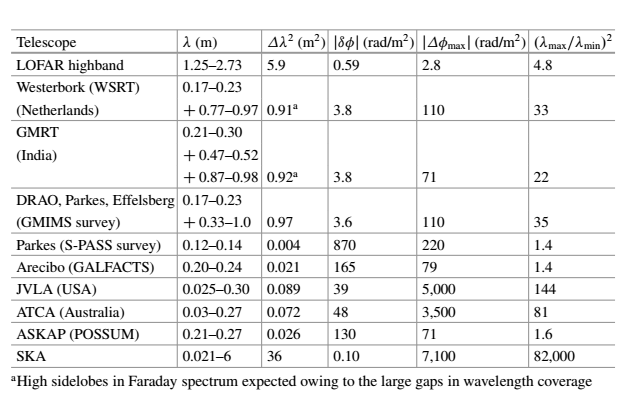
\includegraphics[width=12cm]{figures/RMsynthesis.png}
\end{center}
\end{table}

{\noindent}\textbf{Rotation measure transfer function (RMTF):} A crucially important quantity introduced by de Bruyn (1966) and defined by

\begin{align*}
    R(\phi) \equiv \dfrac{\int\limits_{-\infty}^\infty W(\lambda^2)\mathrm{e}^{-2i\phi(\lambda^2-\lambda_0^2)}\mathrm{d}\lambda^2}{\int\limits_{-\infty}^\infty W(\lambda^2)\mathrm{d}\lambda^2} ~ [{\rm rad\,m^{-2}}],
\end{align*}

{\noindent}which is normalized to unity at $\phi=0$. For a simple weight function $W(\lambda^2)$ that is a top-hat (boxcar) fuction centered on $\lambda_c^2$ with width $\Delta\lambda^2 = \lambda_2^2-\lambda_1^2$, the corresponding RMTF is a sinc function with a phase wind:

\begin{align*}
    R(\phi) = e^{i\phi\lambda_c^2}\left(\dfrac{\sin(\phi\Delta\lambda^2)}{\phi\Delta\lambda^2}\right) ~ [{\rm rad\,m^{-2}}]
\end{align*}

It is a complex valued function; the real part corresponds to the response of the transform parallel to the ($Q,U$) vector at $\lambda_0=\lambda$ while the imaginary part corresponds to the response orthogonal to it. Ideally, the response in the entire main peak of the RMTF should be parallel to the actual polarization vector at $\lambda_0$. Brentjens \& de Bruyn (2005) show that this optimal choice of $\lambda_0^2$ is the mean of the sampled $\lambda^2$ values weighted by $W(\lambda^2)$. However, since the shift theorem of Fourier theory only applies to the argument, changing the value of $\lambda_0$ will not change the absolute value of the RMTF. A drawback of having $\lambda_0\neq0$ is that the polarization angle that one derives still needs to be transformed to a polarization angle at $\lambda=0$ if one wants information on the electric or magnetic field direction of the source. In the case of a high $S/N$, this is easy:

\begin{align*}
    \chi_0 = \chi(\lambda_0^2) - \phi\lambda_0^2 ~ [{\rm rad}].
\end{align*}

{\noindent}However, if the $S/N$ is low, the uncertainty in $\phi$ usually prevents accurate de-rotation to $\lambda=0$. 

{\noindent}\textbf{Second moment:} 

{\noindent}\textbf{Sonic Mach number ($\mathcal{M}_s$):} The sound speed of the \textit{interstellar medium} given by

\begin{align*}
    \mathcal{M}_s = \left\langle\frac{\lvert\vec{v}\rvert}{c_s}\right\rangle ~ [{\rm dimensionless}].
\end{align*}

This number is a commonly used parameter of turbulence used to obtain information on gas compressibility and magnetization. Using polarization gradients of \textit{synchrotron radiation}, it was shown by Gaensler (2011) that the turbulence of the WIM has a relatively low \textit{sonic Mach number}, $\mathcal{M}_s\lesssim2$.

{\noindent}\textbf{Spectral index ($\alpha$):} A measure of the dependence of radiative flux density on frequency. If flux does not follow a power-law distribution, the spectral index itself is a function of frequency. In the radio regime, a spectral index of $\alpha=0-2$ indicates thermal emission while a steep negative spectrum indicates synchrotron radiation.

{\noindent}\textbf{Scintillation:}

{\noindent}\textbf{Spectral correlation function ($S_{x,y}$):} The average over all neighboring spectra of the normalized rms difference between \textit{brightness temperatures} $T_b$ for pairs of velocity channels $(v_i,v_j)$ defined as

\begin{align*}
    S_{x,y} \equiv S_{v_i,v_j} = \frac{1}{n}\sum_{a=1}^n T_b([x,y]_a,v_i)T_b([x,y]_a,v_j),
\end{align*}

{\noindent}where $n$ is the number of positions in the map. A histogram of $S_{x,y}$ reveals the autocorrelation properties: if $S_{x,y}$ is close to unity, the spectra do not vary much.

{\noindent}\textbf{Starlight polarization:} The polarization of initially unpolarized starlight which becomes polarized as it passes through dust grains aligned by an external magnetic field. Paramagnetic materials have unpaired electrons which, when in the presence of an external magnetic field such as the interstellar magnetic field, align in the same direction causing grain alignment. In the case of elongated dust grains, if the shortest axis is aligned with the direction of the magnetic field, then the grains will absorb light polarized along the long axis of the grain which is perpendicular to the field. This results in transmitted radiation having a polarization direction parallel to the magnetic field. Optical polarization of starlight was first imaged by Hall \& Mikesell (1949) and Hiltner (1949). They found that polarized light from nearby stars had similar orientation, indicating that the polarizing mechanism was a source other than the individual stars. Shortly thereafter, Davis \& Greenstein (1951) published a theory on the origin of polarized starlight. They proposed that an elongated dust grain spinning about its shortest axis would have a preferred orientation when located in a magnetic field. Starlight polarization is most useful for detecting magnetic fields in the Solar neighbourhood out to about $1-3\,{\rm kpc}$. The same large-scale alignment of spinning, aspherical dust grains that causes starlight polarization also causes \textit{infrared polarization}.

{\noindent}\textbf{Stellar wind bubble (SWB):} A cavity light years across filled with hot gas blown into the interstellar medium by high-velocity (several thousand ${\rm km\,s^{-1}}$) stellar wind from a single massive O or B star. The heliosphere blown by the Solar wind, within which all of the major planets of the Solar System are embedded, is a small example of a stellar wind bubble.

{\noindent}\textbf{Stochastic system:}

{\noindent}\textbf{Stokes parameters:}

{\noindent}\textbf{Stokes I ($I$):} A measure of the total intensity of radio emission.

{\noindent}\textbf{Stokes Q ($Q$):} A measure of the linear polarization of radio emission. The images of Stokes Q (and \textit{Stokes U}) as well as the \textit{linear polarized intensity} $P\equiv\sqrt{(Q^2+U^2)}$ are often filled with complex structures that bear little resemblance to the \textit{Stokes I} image of total intensity. The intensity variations seen in $Q$ (as well as $U$ and $P$) are the result of small-scale angular structure in the \textit{Faraday rotation} induced by ionized gas, and are thus an indirect representation of turbulent fluctuations in the free-electron density and magnetic field throughout the \textit{interstellar medium}.

{\noindent}\textbf{Stokes U ($U$):} A measure of the linear polarization of radio emission. The images of Stokes U (and \textit{Stokes Q}) as well as the \textit{linear polarized intensity} $P\equiv\sqrt{(Q^2+U^2)}$ are often filled with complex structures that bear little resemblance to the \textit{Stokes I} image of total intensity. The intensity variations seen in $U$ (as well as $Q$ and $P$) are the result of small-scale angular structure in the \textit{Faraday rotation} induced by ionized gas, and are thus an indirect representation of turbulent fluctuations in the free-electron density and magnetic field throughout the \textit{interstellar medium}.

{\noindent}\textbf{Stokes V ($V$):} A measure of circular polarization of radio emission. If $V>0$, then the electromagnetic wave is right-handed circularly polarized (RCP), while if $V<0$, then the electromagnetic wave is left-handed circularly polarized (LCP). Stokes V is related to the line-of-sight magnetic field in the following manner:

\begin{align*}
    V(\nu) \propto B_\parallel \times \frac{\mathrm{d}I}{\mathrm{d}\nu} ~ [{\rm Jy}],
\end{align*}

{\noindent}where $I$ is \textit{Stokes I} and $\nu$ is the observed frequency.

{\noindent}\textbf{Str\"{o}mgren sphere:} A sphere of ionized hydrogen (HII) around young OB stars.

{\noindent}\textbf{Structure function ($S_p(\delta r)$):} The structure function of order $p$ for an observable $A$ is given by

\begin{align*}
    S_p(\delta r) = \langle\lvert A(r)-A(r+\delta r)\rvert^p\rangle,
\end{align*}

{\noindent}for position $r$ and position increment $\delta r$. The power-law fit to this, $S_p(\delta e)\propto\delta r^{\upzeta}_p$, gives the slope $\zeta_p$.

{\noindent}\textbf{Superbubble:} Also known as a \textit{supershell}. A cavity that is hundreds of light years across filled with $1\times10^6\,{\rm K}$ gas blown into the ISM by multiple SNe and stellar winds from clusters and associations of massive O and B stars. A superbubble behaves qualitatively like an individual supernova remnant, except that it has a continuous supply of energy. For the first $3\,{\rm Myrs}$ at least, their energy supply is exclusively due to stellar winds, whose cumulative power rises rapidly with time. Supernovae start exploding after $\gtrsim3\,{\rm Myrs}$, and within $\sim2\,{\rm Myrs}$, they overpower the stellar winds. From then on, the successive supernovae explosions continue to inject energy into the superbubble at a slowly decreasing rate, depending on the \textit{initial mass function} (IMF) of the progenitor stars, until $\sim40\,{\rm Myrs}$. Altogether, stellar winds account for a fraction comprising between $\sim12\%$ and $\sim17\%$ of the total energy input. The Solar System lies near the center of an old superbubble known as the \textit{Local Bubble} whose boundary can be traced by a sudden rise in dust extinction.

{\noindent}\textbf{Supernova:} A supernova is a transient astronomical event that occurs during the last stellar evolutionary stages of a star's life, either a massive star or a white dwarf, whose destruction is marked by one final, titanic explosion. Supernovae come in two types. \textit{Type-I} supernovae arise from old, degenerate low-mass stars which supposedly are accreting from a companion and undergoes a thermonuclear instability upon accumulation of a critical mass. \textit{Type-II} supernovae arise from young stars with initial masses $\gtrsim8\,{\rm M}_\odot$ whose core gravitationally collapses once it has exhausted all of its fuel. Like the bright, massive stars, Type-II supernovae are tightly confined to the spiral arms while Type-I supernovae have a more spread-out distribution similar to the general stellar population. Type-I supernovae are less frequent than their Type-II counterparts. All of them are uncorrelated in space and have basically the same repercussions on the ISM as isolated Type-II supernovae. The hot gas created by supernovae explosions (and stellar winds) in the Galactic disk rises into the halo under the influence of its own buoyancy. In the course of its upward motion, it cools down (almost adiabatically at first, then by radiative transport), and eventually condenses into cold neutral clouds. Once formed, these clouds fall ballistically towards the Galactic plane. This convective cycle of interstellar material between the disk and the halo is known as the \textit{Galactic fountain}.

{\noindent}\textbf{Synchrotron radiation:} The radio emission produced by relativistic \textit{cosmic rays} when accelerated radially (e.g., by magnetic fields) which is one of the most commonly used tracers of the Galactic magnetic field. Synchrotron emission has a steep spectral index of $\alpha\sim-2.75$, which results in much brighter emission at lower frequencies (this applies to both linear polarization and total intensity). For a single electron, the critical frequency of synchrotron radiation can be expressed as

\begin{align*}
    \nu_c = \dfrac{3}{4\pi}\dfrac{q}{mc}\gamma^2(B\sin\theta)~[{\rm Hz}],
\end{align*}

{\noindent} or

\begin{align*}
\nu_c \sim \gamma^2 \frac{eB}{2\pi m_0} ~ [{\rm Hz}],
\end{align*}

{\noindent}where $\gamma$ is the \textit{Lorentz factor}, $e$ and $m_0$ are the charge and rest mass of the cosmic ray electron, and $B$ is the magnetic field strength. As the cosmic ray gyrates around the local magnetic field, it generates the synchrotron radiation beamed within the shape of a cone at an angle of 

\begin{align*}
    \theta = \pm \frac{m_cc^2}{E} ~ [{\rm rad}].
\end{align*}

{\noindent}On the surface of the cone, the radiation is 100\% linearly polarized with an electric field $E$ that has a direction of $-\mathbf{v\times B}$. Synchrotron radiation from the Galaxy was the first emission detected in radio astronomy by Jansky (1933), however, it was not until the 1950's when detailed radio maps of the Galaxy were produced that the connection was made between radio emission and the synchrotron mechanism. Linear polarization of synchrotron radiation can be used to trace ordered magnetic fields in the plane of the sky ($B_\perp$). Unpolarized synchrotron emission can be indicative of a turbulent magnetic field causing depolarization via Faraday rotation of thermal electrons (synchrotron radiation cannot cause Faraday rotation). The radiated power from an accelerating charge $q$ with mass $m$ by a magnetic field $B$ at an observing frequency $\nu$ is

\begin{align*}
    P = \frac{2}{3}\dfrac{q^4}{m^2c^5}(\gamma\nu)^2(B\sin\theta)^2 ~ [{\rm Jy}].
\end{align*}

{\noindent}Since synchrotron radiation is proportional to the charge-to-mass ratio, electrons dominate synchrotron radiation over protons and ions by several orders of magnitude. Synchrotron radiation peaks at a characteristic frequency of

\begin{align*}
    \nu_c = \dfrac{3}{4\pi}\dfrac{q}{mc}\gamma^2(B\sin\theta)~[{\rm Hz}].
\end{align*}

{\noindent}For radio observations with typical frequencies at or above tens of ${\rm MHz}$ and with typical magnetic field strengths of order $\mu$G, the observed population of synchrotron electrons have $\gamma\gg1$. Synchrotron emission has a steep negative spectral index in the radio regime. Assuming that the electrons are moving isotropically, Le Roux (1961) showed that the maximum intrinsic degree of polarization (i.e., polarization fraction) of synchrotron radiation from plasma in a uniform magnetic field is a function of the electron's spectral index $\gamma$ given by

\begin{align*}
    p = \frac{3\gamma + 3}{3\gamma+7} ~ [{\rm dimensionless}],
\end{align*}

{\noindent}independent of frequency and observing angle. Using observations of the Crab Nebula, Woltjer (1958) and Westfold (1959) showed that $\gamma\approx5/3$ and therefore $p\approx67\%$. Le Roux (1961) gives a full derivation of synchrotron radiation. Figure \ref{figure:408mhz} shows the Galactic synchrotron emission at $408\,{\rm MHz}$.

\begin{figure}[h]
\begin{center}
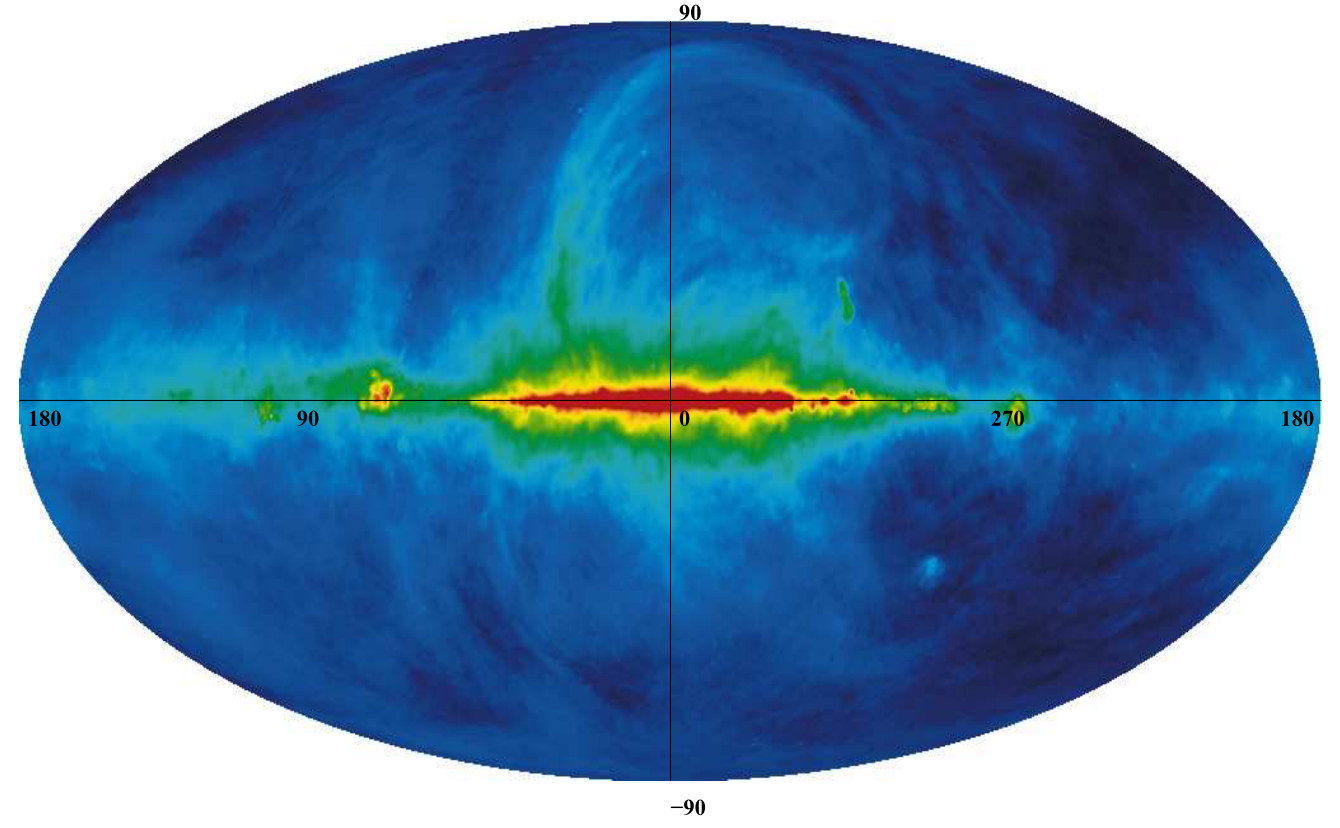
\includegraphics[width=15cm]{figures/408MHz.png}
\caption{The synchrotron emission at $408\,{\rm MHz}$ across the entire sky in Galactic coordinates. As expected, the emission is concentrated along the Galactic plane. However, the feature known as Loop I, is clearly arching up from $\ell=55^\circ$ towards the North Galactic Pole. This Figure is adapted from Haslam et al. (1981). Figure taken from Newton-McGee (2009).}
\label{figure:408mhz}
\end{center}
\end{figure}

{\noindent}\textbf{Tangential component of polarization gradient:}

\begin{align*}
    \frac{\partial\mathbf{P}}{\partial s}_\mathrm{rad} = \sqrt{\frac{(Q\frac{\partial U}{\partial x} - U\frac{\partial Q}{\partial x})^2 + (Q\frac{\partial U}{\partial y} - U\frac{\partial Q}{\partial y})^2}{Q^2+U^2}} ~ [{\rm Jy\,pc^{-1}}]
\end{align*}

{\noindent}\textbf{Taylor scale:}

{\noindent}\textbf{Tsallis distribution:} A function that can be fit to incremental probability distribution functions (PDFs) of turbulent density, magnetic field, and velocity. The Tsallis distribution was originally derived by Tsallis (1988) as a means to extend traditional Boltzmann-Gibbs mechanics to fractal and multifractal systems. The complex dynamics of multifractal systems apply to many natural environments, such as ISM turbulence. The Tsallis function of an arbitrary incremental PDF $\Delta f$ has the form

\begin{align*}
    R_q = a \left[ 1+(q-1) \dfrac{\Delta f(r)^2}{w^2} \right]^{-1/(q-1)}.
\end{align*}

{\noindent}The fit is described by three dependent variables. The $a$ parameter describes the amplitude while $w$ is related to the width or dispersion of the distribution. Parameter $q$, referred to as the ``non-extensivity parameter'' or ``entropic index'' describes the sharpness and tail size of the distribution. The Tsallis fit parameters are in many ways similar to statistical moments. Moments, more specifically the third- and fourth-order moments, have been used to describe the density distributions and have shown sensitivities to simulation compressibility. The first- and second-order moments simply correspond to the mean and variance of a distribution. Skewness, or third-order moment, describes the asymmetry of a distribution about its mode. Skewness can have positive or negative values corresponding to right and left shifts of a distribution, respectively. The fourth-order moment, kurtosis, is a measure of a distribution’s peaked or flatness compared to a Gaussian distribution. Like skewness, kurtosis can have positive or negative values corresponding to increased sharpness or flatness. With regard to the Tsallis fitting parameters, the w parameter is similar to the second-order moment variance while q is closely analogous to fourth-order moment kurtosis. Unlike higher order moments, however, the Tsallis fitting parameters are dependent least-squares fit coefficients and are more sensitive to subtle changes in the PDF.

{\noindent}\textbf{Turbulence:} Astrophysical turbulence is a complex nonlinear fluid phenomenon that can occur in a multiphase medium which results in the excitation of an extreme range of correlated spatial and temporal scales. There are many injection sources on scales ranging from ${\rm kp}$ down to sub-${\rm AU}$ The physical processes by which kinetic energy is converted into turbulence are not well understood for the ISM. The main sources for large-scale motions are: (a) stars, whose energy input is in the form of protostellar winds, expanding HII regions, O star and Wolf-Rayet winds, supernovae, and combinations of these producing superbubbles; (b) Galactic rotation in the shocks of spiral arms or bars, in the \textit{Balbus-Hawley instability} (also known as the magnetorotational instability), and in the gravitational scattering of cloud complexes at different epicyclic phases; (c) gaseous self-gravity through swing-amplified instabilities and cloud collapse; (d) \textit{Kelvin-Helmholtz} and other fluid instabilities; and (e) Galactic gravity during disk-halo circulation, the \textit{Parker instability}, and galaxy interactions. Interstellar turbulence has been characterized by \textit{structure functions}, \textit{autocorrelations}, \textit{power spectra}, \textit{energy spectra}, and \textit{delta variance}. Sources for small-scale turbulence observed by radio \textit{scintillation} include sonic reflections of shock waves hitting clouds, cosmic ray streaming and other instabilities, field star motions and winds, and energy cascades from larger scales. Turbulence affects the structure and motion of nearly all temperature and density regimes of the interstellar gas. Magnetohydrodynamic (MHD) turbulence is a key element in the study of star formation, molecular cloud structure, magnetic reconnection, heat transport, and cosmic ray propagation. MHD turbulence is known to be different from a collection of linear Alfv\'enic waves. Does MHD turbulence, specifically the Alfv\'en wave modes, damp at the decoupling scale of the \textit{ambipolar diffusion scale} $L_\mathrm{AD}$? Cascading rates and the anisotropy of turbulence should be accounted for carefully before a definitive conclusion about turbulent damping in the partially ionized media. Despite the importance of turbulence for ISM studies, many mysteries remain including the nature of turbulence driving and damping. The most common observational techniques for studying turbulence include scintillation studies (which are limited to fluctuations in ionized plasmas), density fluctuations via column density maps, and radio spectroscopic observations via centroids of spectral lines. Position-position-velocity (PPV) spectroscopic data have the advantage over column density maps in that it contains information on the turbulent velocity field. However, this type of data provides contributions of both velocity and density fluctuations entangled together, and the process of separating the two has proven to be a challenging problem. One of the main approaches for characterizing ISM turbulence is based on using statistical techniques and descriptions (e.g., spatial power spectrum). Although the power spectrum is useful for obtaining information about energy transfer over scales, it does not provide a full picture of turbulence, partly because it only contains information on Fourier amplitudes (i.e., two substantially different density distributions can have the same power spectrum). Probability distribution functions (PDFs) of turbulence in PPV and column density data have been studied for decades and have proven to be very useful to show that turbulence is present in the ISM, providing insight into the effects of turbulent driving and characterizing the type of turbulence in question. Many studies on turbulence focus on obtaining parameters such as \textit{sonic and Alfv\'en Mach numbers}, \textit{injection scale}, gas temperature, and \textit{Reynolds number}. In particular, the sonic and Alfv\'en Mach numbers provide much coveted information on the gas compressibility and magnetization.

{\noindent}\textbf{Turbulent fragmentation:}

{\noindent}\textbf{Turbulent magnetic field:} Also known as a random magnetic field.

{\noindent}\textbf{Turbulent pressure:}

{\noindent}\textbf{Two-fluid turbulence:} The turbulence of a partially ionized plasma where the ions are decoupled from the neutrals (i.e., at the scale below the \textit{ambipolar diffusion scale}).

{\noindent}\textbf{Type-I Supernova:} Arises from old, degenerate low-mass stars which supposedly are accreting from a companion and undergoes a thermonuclear instability upon accumulation of a critical mass. Like Type-II supernovae, releases an amount of energy of $\simeq10^{51}\,{\rm ergs}$.

{\noindent}\textbf{Type-II Supernova:} Arises from young stars with initial masses $\gtrsim8\,{\rm M}_\odot$ whose core gravitationally collapses once it has exhausted all of its fuel. Like Type-I supernovae, releases an amount of energy of $\simeq10^{51}\,{\rm ergs}$.

{\noindent}\textbf{Volume filling factor ($f$):} A correction factor such that a fraction $f$ of the line of sight intersects clouds of uniform density $N$. There are three effects of the interstellar magnetic field that conspire to lower the filling factor of hot cavities: (1) the background magnetic pressure acting on the surrounding shells directly opposes their expansion, (2) the magnetic tension in the swept-up field lines gives rise to an inward restoring force, while the associated magnetic pressure prevents the shells from fully collapsing and, therefore, keeps them relatively thick, and (3) the enhanced external ``signal speed'' causes the shells to merge earlier than they would in an unmagnetized medium.

{\noindent}\textbf{Warm ionized medium (WIM):} A diffuse phase of the \textit{interstellar medium} with a typical temperature of $T\sim8,000\,{\rm K}$ and average electron density of $\sim0.2-0.5\,{\rm cm^{-3}}$. The ionized gas has mostly been mapped using the H$\alpha$ line. One limitation of the H$\alpha$ line comes from the obscuration caused by dust, which restricts visibility to within $2-3\,{\rm kpc}$ from the Sun. Using polarization gradients of \textit{synchrotron radiation}, it was shown by Gaensler (2011) that the turbulence of the WIM has a relatively low \textit{sonic Mach number}, $\mathcal{M}_s\lesssim2$.

{\noindent}\textbf{Warm partially ionized medium (WPIM):}

{\noindent}\textbf{Wave turbulence:}

{\noindent}\textbf{Zeeman effect:} The effect of a single spectral line splitting into multiple components in the presence of a static magnetic field due to the degeneracy between various electron energy levels that become broken when exposed to an external magnetic field. In an astrophysical context, a magnetic field produces small frequency shifts in the left- and right-handed circular polarized components of a given spectral line with respect to the intrinsic central frequency of the atom of molecule. Zeeman splitting is used to measure the parallel component of the magnetic field via atomic and molecular gas. The first measurement of an astrophysical magnetic field was using Zeeman splitting. The $21\,{\rm cm}$ line of atomic hydrogen is the most widespread, and it provides an opportunity to measure splitting in both emission and absorption. Zeeman splitting is a powerful tool as the magnetic field can be directly determined from the energy difference between the electron levels. The separation in energy of the magnetic hyperfine levels from the unsplit level of the zero magnetic field case is given by

\begin{align*}
    \Delta E = -\mu_Bm_FgB ~ [{\rm J}],
\end{align*}

{\noindent}where $\mu_B$ is the Bohr magneton, $m_F$ is the quantum number of the Zeeman splitting, $B$ is the magnetic field strength, and $g$ is the Land\'e g-factor. However, the effect is difficult to observe since the frequency shift ($\Delta\nu$) in the spectral lines is small:

\begin{align*}
    \Delta\nu = \frac{\mu_Bm_FgB}{h} ~ [{\rm Hz}].
\end{align*}

{\noindent}Such a frequency shift is usually smaller than the spectral linewidth, making Zeeman splitting observations resolution limited. Lower frequencies produce better Zeeman splitting results because, although the splitting is independent of the line frequency itself, the higher the frequency, the broader the linewidth.

{\noindent}\textbf{Zenith:} The point in the sky or celestial sphere directly above an observer.

{\noindent}\textbf{Zeroth moment:} 








































%%%%%%%%%%%%%%%%%%%%%%%%
%                                                                       %
%                     PARAMETERS                          %
%                                                                       %
%%%%%%%%%%%%%%%%%%%%%%%%

\newpage
\section{Parameters}

{\noindent}\textbf{Alfv\'en Mach number}: $\mathcal{M}_A~[{\rm dimensionless}]$

{\noindent}\textbf{Alfv\'en speed}: $v_A~[{\rm m\,s^{-1}}]$

{\noindent}\textbf{Ambipolar diffusion scale}: $L_\mathrm{AD}~[{\rm m}]$

{\noindent}\textbf{Ambipolar diffusivity}: $\nu_\mathrm{AD}$

{\noindent}\textbf{Angle}: $\theta~[{\rm rad}]$

{\noindent}\textbf{Autocorrelation}: $C(\delta r)~[{\rm dimensionless}]$

{\noindent}\textbf{Bandwidth in frequency}: $\Delta\nu~[{\rm Hz}]$

{\noindent}\textbf{Bandwidth in wavelength}: $\Delta\lambda~[{\rm Hz}]$

{\noindent}\textbf{Bohr magneton}: $\mu_B$

{\noindent}\textbf{Channel central frequency}: $\nu_c~[{\rm Hz}]$

{\noindent}\textbf{Channel width in frequency}: $\delta\nu~[{\rm Hz}]$

{\noindent}\textbf{Channel central wavelength}: $\lambda_c~[{\rm m}]$

{\noindent}\textbf{Channel width in wavelength}: $\delta\lambda~[{\rm m}]$

{\noindent}\textbf{Complex conjugate}: ${f(x)}^*\,{\rm or}\,\bar{f}(x)$

{\noindent}\textbf{Delta function}: $\delta (x)$

{\noindent}\textbf{Delta variance}: $\sigma_\Delta^2(L)$

{\noindent}\textbf{Density}: $\rho~[{\rm m^{-3}}]$

{\noindent}\textbf{Density of electrons}: $\rho_e~[{\rm m^{-3}}]$

{\noindent}\textbf{Density of ions}: $\rho_i~[{\rm m^{-3}}]$

{\noindent}\textbf{Density of neutrals}: $\rho_n~[{\rm m^{-3}}]$

{\noindent}\textbf{Diameter of window (RHT)}: $D_W ~ [{\rm pixels}]$

{\noindent}\textbf{Dirac delta function}: $\delta(x)$

{\noindent}\textbf{Dispersion measure}: ${\rm DM} ~ [{\rm pc\,cm^{-3}}]$

{\noindent}\textbf{Electron charge}: $e~[{\rm C}]$

{\noindent}\textbf{Electron mass}: $e_m~[{\rm kg}]$

{\noindent}\textbf{Emission measure}: ${\rm EM} ~ [{\rm pc\,cm^{-6}}]$

{\noindent}\textbf{Energy spectrum}: $E(k)~[{\rm Jy\,m^{-1}}]$

{\noindent}\textbf{Expectation value of $\theta$ on any domain (RHT)}: $\langle\theta\rangle' ~ [{\rm rad}]$

{\noindent}\textbf{Expectation value of $\theta$ on $\theta\in[0,\pi)$ (RHT)}: $\langle\theta\rangle ~ [{\rm rad}]$

{\noindent}\textbf{Faraday depth}: $\phi~[{\rm rad\,m^{-2}}]$

{\noindent}\textbf{Faraday dispersion function (no spectral dependence)}: $F(\phi)~[{\rm rad\,m^{-2}}]$

{\noindent}\textbf{Faraday dispersion function (general form)}: $F(\phi,\lambda)~[{\rm rad\,m^{-2}}]$

{\noindent}\textbf{Frequency}: $\nu~[{\rm Hz}]$

{\noindent}\textbf{Frictional coupling coefficient between ions and neutrals}: $\alpha~[{\rm dimensionless}]$

{\noindent}\textbf{FWHM of RMTF main peak}: $\Delta\phi~[{\rm rad\,m^{-2}}]$

{\noindent}\textbf{Fourier transform (FT)}: $\hat{f}(x)$

{\noindent}\textbf{Incremental position}: $\delta r~[{\rm m}]$

{\noindent}\textbf{Intensity threshold}: $Z ~ [{\rm dimensionless}]$

{\noindent}\textbf{Jansky}: $\mathrm{Jy} ~ [\rm unit]$

{\noindent}\textbf{Joule}: $\mathrm{J} ~ [\rm unit]$

{\noindent}\textbf{Diameter of kernel (RHT)}: $D_K ~ [{\rm pixels}]$

{\noindent}\textbf{Land\'e g-factor}: $g$

{\noindent}\textbf{Lorentz factor}: $\gamma ~ [\rm dimensionless]$

{\noindent}\textbf{Mach number}: $\mathcal{M}~[{\rm dimensionless]}$

{\noindent}\textbf{Magnetic field strength}: $B~[{\rm \mu G]}$

{\noindent}\textbf{Number of $\theta$ bins (RHT)}: $n ~ [{\rm dimensionless}]$

{\noindent}\textbf{Order}: $p~[{\rm dimensionless}]$

{\noindent}\textbf{Planck constant}: $h~[{\rm J\,s}]$

{\noindent}\textbf{Planck constant (reduced)}: $\hbar~[{\rm J\,s}]$

{\noindent}\textbf{Polarization angle}: $\chi~[{\rm rad}]$

{\noindent}\textbf{Polarization angle (RHT)}: $\chi_\mathrm{RHT} ~ [{\rm rad}]$

{\noindent}\textbf{Polarization angle at $\lambda=0$}: $\chi_0~[{\rm rad}]$

{\noindent}\textbf{Polarization fraction}: $p(\lambda^2)~[{\rm dimensionless}]$

{\noindent}\textbf{Polarization gradient}: $\lvert\nabla \mathbf{P}\rvert ~ [\rm Jy\,beam^{-1}]$

{\noindent}\textbf{Polarization gradient direction}: $\mathrm{arg}(\nabla\mathbf{P}) ~ [\rm rad]$

{\noindent}\textbf{Polarized intensity}: $P ~ [\rm Jy]$

{\noindent}\textbf{Polarized surface brightness}: $P(\lambda^2) ~ [\rm Jy]$

{\noindent}\textbf{Polarized surface brightness (observed)}: $\tilde{P}(\lambda^2) ~ [\rm Jy]$

{\noindent}\textbf{Position}: $r~[{\rm m}]$

{\noindent}\textbf{Power spectrum}: $P(k)$

{\noindent}\textbf{Quantum number of Zeeman splitting}: $m_F$

{\noindent}\textbf{Radial component of polarization gradient}: $\dfrac{\partial\mathbf{P}}{\partial s}_\mathrm{rad} ~ [{\rm Jy\,pc^{-1}}]$

{\noindent}\textbf{Rest mass}: $m_0~[{\rm kg}]$

{\noindent}\textbf{Reynolds number}: $R~[{\rm dimensionless}]$

{\noindent}\textbf{Reynolds number for ambipolar diffusion}: $R_\mathrm{AD}~[{\rm dimensionless}]$

{\noindent}\textbf{RHT angle}: $\theta~[{\rm rad}]$

{\noindent}\textbf{RHT backprojection}: $R(x,y) ~ [{\rm dimensionless}]$

{\noindent}\textbf{RHT backprojection sampling disk around star}: $R_*(x,y) ~ [{\rm dimensionless}]$

{\noindent}\textbf{RHT distance}: $\rho~[{\rm pixels}]$

{\noindent}\textbf{RHT intensity vs angle}: $R(\theta,x_0,y_0)~[{\rm dimensionless}]$

{\noindent}\textbf{Rotation measure}: ${\rm RM~[rad\,m^{-2}]}$

{\noindent}\textbf{Rotation measure transfer function (RMTF)}: $R(\phi) {\rm [rad\,m^{-2}]}$

{\noindent}\textbf{Sonic Mach number}: $\mathcal{M}_s~[{\rm dimensionless]}$

{\noindent}\textbf{Sound speed}: $c_s ~ [{\rm m\,s^{-1}}]$

{\noindent}\textbf{Spectral correlation function}: $S_{x,y}~[\rm{dimensionless}]$

{\noindent}\textbf{Spectral index}: $\alpha~[\rm{dimensionless}]$

{\noindent}\textbf{Speed of light}: $c~[\rm{m\,s^{-1}}]$

{\noindent}\textbf{Standard deviation}: $\sigma(x)$

{\noindent}\textbf{Stokes I}: $I ~ [\rm Jy]$

{\noindent}\textbf{Stokes Q}: $Q ~ [\rm Jy]$

{\noindent}\textbf{Stokes Q (RHT)}: $Q_\mathrm{RHT} ~ [\rm Jy]$

{\noindent}\textbf{Stokes U}: $U ~ [\rm Jy]$

{\noindent}\textbf{Stokes U (RHT)}: $U_\mathrm{RHT} ~ [\rm Jy]$

{\noindent}\textbf{Stokes V}: $V ~ [\rm Jy]$

{\noindent}\textbf{Structure function}: $S_p$

{\noindent}\textbf{Structure function power-law slope}: $\zeta_p$

{\noindent}\textbf{Tangential component of polarization gradient}: $\dfrac{\partial\mathbf{P}}{\partial s}_\mathrm{tan} ~ [{\rm Jy\,pc^{-1}}]$

{\noindent}\textbf{Variance}: $\sigma^2$

{\noindent}\textbf{Wavelength}: $\lambda~[{\rm m}]$

{\noindent}\textbf{Wavelength to which all polarization vectors are de-rotated}: $\lambda_0~[{\rm m}]$

{\noindent}\textbf{Wavenumber}: $k~[{\rm m^{-1}}]$

{\noindent}\textbf{Weight function}: $W(\lambda^2)~[\rm{dimensionless}]$

{\noindent}\textbf{Zeeman splitting energy difference}: $\Delta E ~ [{\rm J}]$

{\noindent}\textbf{Zeeman splitting frequency difference}: $\Delta \nu ~ [{\rm Hz}]$








































%%%%%%%%%%%%%%%%%%%%
%                                                          %
%                      EQUATIONS               %
%                                                          %
%%%%%%%%%%%%%%%%%%%%

\newpage
\section{Equations}

{\noindent}\textbf{Alfv\'en Mach number:}
\begin{align*}
    \mathcal{M}_A = \left\langle\frac{\lvert\vec{v}\rvert}{v_A}\right\rangle ~ [{\rm dimensionless}]
\end{align*}

{\noindent}\textbf{Alfv\'en speed:}
\begin{align*}
    v_A = \frac{\lvert\vec{B}\lvert}{\sqrt{\rho}} ~ [{\rm m\,s^{-1}}]
\end{align*}

{\noindent}\textbf{Ambipolar diffusion scale:}
\begin{align*}
    L_\mathrm{AD} = \dfrac{V_A}{\alpha\rho_i} ~ [\rm m]
\end{align*}

{\noindent}\textbf{Ambipolar diffusivity:}
\begin{align*}
    \nu_\mathrm{AD} = \dfrac{B^2}{4\pi\rho_i\rho_n\alpha} ~ [{\rm m^s\,s^{-1}}]
\end{align*}

{\noindent}\textbf{Autocorrelation:}
\begin{align*}
    C(\delta r) = \langle f(r)f(r+\delta r)\rangle ~ [{\rm dimensionless}].
\end{align*}

{\noindent}\textbf{Channel central wavelength:} 
\begin{align*}
\lambda_c^2 \approx \dfrac{c^2}{\nu_c^2} \left(1+\dfrac{3}{4}\left(\dfrac{\delta\nu}{\nu_c}\right)^2\right) ~ [{\rm m^2}]
\end{align*}
(Brentjens \& de Bruyn, 2005)

{\noindent}\textbf{Channel width in wavelength:} 
\begin{align*}
\delta\lambda^2 \approx \dfrac{2c^2\delta\nu}{\nu_c^3} \left(1+\dfrac{1}{2}\left(\dfrac{\delta\nu}{\nu_c}\right)^2\right) ~ [{\rm m^2}]
\end{align*}
(Brentjens \& de Bruyn, 2005)

{\noindent}\textbf{Delta variance:}
\begin{align*}
    \sigma_\Delta^2(L) = \left\langle \int\limits_0^{3L/2} {(A[r+x]-\langle A\rangle)\odot(x)}^2\mathrm{d}x \right\rangle,
\end{align*}

{\noindent}\textbf{Dispersion measure (DM):}
\begin{align*}
    {\rm DM} = -\int\limits_\mathrm{source}^\mathrm{observer} n_e\vec{{\rm d}\ell} ~ [{\rm pc\,cm^{-3}}]
\end{align*}

{\noindent}\textbf{Emission measure:}
\begin{align*}
    {\rm EM} = -\int\limits_\mathrm{source}^\mathrm{observer} n_e^2\vec{{\rm d}\ell} ~ [{\rm pc\,cm^{-6}}]
\end{align*}

{\noindent}\textbf{Expectation value of $\theta$ on any domain (RHT):}
\begin{align*}
    \langle\theta\rangle' = \frac{1}{2}\arctan \left[\frac{\int\sin(2\theta)R_*(\theta)\mathrm{d}\theta}{\int\cos(2\theta)R_*(\theta)\mathrm{d}\theta}\right]
\end{align*}

{\noindent}\textbf{Expectation value of $\theta$ on $\theta\in[0,\pi)$ (RHT):}
\begin{align*}
    \langle\theta\rangle = \pi - {\rm mod}(\langle\theta\rangle'+\pi,\pi) ~ [{\rm rad}]
\end{align*}

{\noindent}\textbf{Faraday depth:} 
\begin{align*}
    \phi(\vec{r}) = -0.81 \int\limits_\mathrm{source}^\mathrm{observer}n_e\vec{B}\cdot\vec{{\rm d}r} ~ [{\rm rad\,m^{-2}}]
\end{align*}

{\noindent}\textbf{Faraday depth standard error:}
\begin{align*}
\sigma_\phi &= \left[ \dfrac{1}{N-2} \dfrac{\sum_i\chi_i^2}{\sum_i(\lambda_i^2)^2 - N^{-1}(\sum_i\lambda_i^2)^2} \right]^{-1} \\
&= \left[ \dfrac{1}{N-2} \dfrac{(N-1)(\sigma_\chi^2 + \cancel{\langle\chi\rangle})}{\sum_i(\lambda_i^2)^2 - N^{-1}(\sum_i\lambda_i^2)^2} \right]^{-1} \\
&= \left[ \dfrac{N-1}{N-2} \dfrac{\sigma_\chi^2}{\sum_i(\lambda_i^2)^2 - N^{-1}(\sum_i\lambda_i^2)^2} \right]^{-1} \\
&\approx \left[ \dfrac{\sigma_Q^2\approx\sigma_U^2\approx\sigma^2}{4(N-2)\lvert\lvert P \rvert\rvert^2\sigma_{\lambda^2}^2} \right]^{-1} ~ [{\rm rad\,m^{-2}}]
\end{align*}
(Brentjens \& de Bruyn, 2005)

{\noindent}\textbf{Faraday dispersion function:}
\begin{align*}
F(\phi) = \int\limits_{\infty}^\infty P(\lambda^2)\mathrm{e}^{-2i\phi\lambda^2}\mathrm{d}\lambda^2 ~ [{\rm rad\,m^{-2}}]
\end{align*}

{\noindent}\textbf{Faraday dispersion function (reconstructed):}
\begin{align*}
\tilde{F}(\phi) \equiv \dfrac{\int\limits_{-\infty}^\infty \tilde{P}(\lambda^2)\mathrm{e}^{-2i\phi(\lambda^2-\lambda_0^2)}\mathrm{d}\lambda^2}{\int\limits_{-\infty}^\infty W(\lambda^2)\mathrm{d}\lambda^2} = F(\phi) * R(\phi) ~ [{\rm rad\,m^{-2}}]
\end{align*}

{\noindent}\textbf{Fourier transform (FT):}
\begin{align*}
    \hat{f}(x) = \int\limits_{-\infty}^\infty f(x')e^{-2\pi xx'}dx'
\end{align*}

{\noindent}\textbf{Inverse Fourier transform (FT):}
\begin{align*}
    f(x) = \int\limits_{-\infty}^\infty \hat{f}(x')e^{2\pi ixx'}dx'
\end{align*}

{\noindent}\textbf{Lorentz factor:}
\begin{align*}
    \gamma = \sqrt{\frac{1 - (v/c)^2}{c^2}} ~ [{\rm dimensionless}]
\end{align*}

{\noindent}\textbf{Number of $\theta$ bins (RHT):}
\begin{align*}
    n_\theta = \left[\pi\frac{\sqrt{2}}{2}(D_W-1)\right] ~ [{\rm dimensionless}]
\end{align*}

{\noindent}\textbf{Polarization angle:}
\begin{align*}
\chi &= \dfrac{1}{2}\arctan\left(\dfrac{U}{Q}\right) ~ [{\rm rad}] \\
&= \chi_0 + \mathrm{RM}\lambda^2 ~ [{\rm rad}]
\end{align*}

{\noindent}\textbf{Polarization angle (RHT):}
\begin{align*}
\chi_\mathrm{RHT} = \dfrac{1}{2}\arctan\left(\dfrac{U_\mathrm{RHT}}{Q_\mathrm{RHT}}\right) ~ [{\rm rad}]
\end{align*}

{\noindent}\textbf{Polarization angle distribution standard error:} 
\begin{align*}
\sigma_\chi = \left[ \dfrac{1}{N-1} \sum_i\chi_i^2 - \langle\chi\rangle \right]^{-1} ~ [{\rm rad}]
\end{align*}
(Brentjens \& de Bruyn, 2005)

{\noindent}\textbf{Polarization angle standard error:}
\begin{align*}
\sigma_\chi &= \sqrt{ \left(\dfrac{\partial\chi}{\partial Q}\right)^2\sigma_Q^2 + \left(\dfrac{\partial\chi}{\partial U}\right)^2\sigma_U^2 }\\
&= \sqrt{ \left(\dfrac{\partial\frac{1}{2}\arctan\frac{U}{Q}}{\partial Q}\right)^2\sigma_Q^2 + \left(\dfrac{\partial\frac{1}{2}\arctan\frac{U}{Q}}{\partial U}\right)^2\sigma_U^2 } \\
&= \sqrt{ \left(\dfrac{1}{4}\dfrac{U^2}{(Q^2+U^2)^2}\right)\sigma_Q^2 + \left(\dfrac{1}{4}\dfrac{Q^2}{(Q^2+U^2)^2}\right)\sigma_U^2 } \\
&= \dfrac{U^2\sigma_Q^2 + Q^2\sigma_U^2}{4\lvert\lvert P \rvert\rvert^4} ~ [{\rm rad}]
\end{align*}
(Brentjens \& de Bruyn, 2005)

{\noindent}\textbf{Polarization angle at $\lambda=0$ standard error:} 
\begin{align*}
\sigma_{\chi_0} = \left[ \dfrac{\sigma_Q^2\approx\sigma_U^2\approx\sigma^2}{4(N-2)\lvert\lvert P \rvert\rvert^2} \left( \dfrac{N-1}{N} + \dfrac{\lambda_0^4}{\sigma_{\lambda^2}^2} \right) \right]^{-1} ~ [{\rm rad}]
\end{align*}
(Brentjens \& de Bruyn, 2005)

{\noindent}\textbf{Polarization fraction:}
\begin{align*}
p(\lambda^2) = \dfrac{P(\lambda^2)}{I(\lambda^2)} ~ [{\rm dimensionless}]
\end{align*}

{\noindent}\textbf{Polarization gradient:}
\begin{align*}
    \lvert\nabla \mathbf{P}\rvert = \sqrt{\left(\frac{\partial Q}{\partial x}\right)^2 + \left(\frac{\partial U}{\partial x}\right)^2 + \left(\frac{\partial Q}{\partial y}\right)^2 + \left(\frac{\partial U}{\partial y}\right)^2} ~ [\rm Jy\,beam^{-1}]
\end{align*}

{\noindent}\textbf{Polarization gradient direction:}
\begin{align*}
    \mathrm{arg}(\nabla\mathbf{P}) \equiv \arctan \left[ \mathrm{sign} \left(\dfrac{\partial Q}{\partial x}\dfrac{\partial Q}{\partial y} + \dfrac{\partial U}{\partial x}\dfrac{\partial U}{\partial y}\right) \dfrac{\sqrt{\left(\dfrac{\partial Q}{\partial y}\right)^2 + \left(\dfrac{\partial U}{\partial y}\right)^2}}{\sqrt{\left(\dfrac{\partial Q}{\partial x}\right)^2 + \left(\dfrac{\partial U}{\partial x}\right)^2}} \right] ~ [\rm rad]
\end{align*}

{\noindent}\textbf{Polarized intensity:}
\begin{align*}
    P\equiv\sqrt{Q^2+U^2} ~ [\rm Jy]
\end{align*}

{\noindent}\textbf{Polarized intensity standard error:}
\begin{align*}
\sigma_P &= \sqrt{ \left(\dfrac{\partial\lvert\lvert P \rvert\rvert}{\partial Q}\right)^2\sigma_Q^2 + \left(\dfrac{\partial\lvert\lvert P \rvert\rvert}{\partial U}\right)^2\sigma_U^2 } \\
&= \sqrt{ \left(\dfrac{Q^2}{Q^2+U^2}\right)\sigma_Q^2 + \left(\dfrac{U^2}{Q^2+U^2}\right)\sigma_U^2 } \\
&= \sqrt{ \dfrac{Q^2}{\lvert\lvert P \rvert\rvert^2}\sigma_Q^2 + \dfrac{U^2}{\lvert\lvert P \rvert\rvert^2}\sigma_U^2 } ~ [\rm Jy]
\end{align*}
(Brentjens \& de Bruyn, 2005)

{\noindent}\textbf{Polarized surface brightness:}
\begin{align*}
P(\lambda^2) &= \lvert\lvert p(\lambda^2) \rvert\rvert I\mathrm{e}^{2i\chi} = p(\lambda^2)I(\lambda^2) = Q+iU ~ [\rm Jy] \\
&= \int\limits_{-\infty}^\infty F(\phi)\mathrm{e}^{2i\phi\lambda^2}\mathrm{d}\phi ~ [\rm Jy]
\end{align*}

{\noindent}\textbf{Polarized surface brightness (absolute):}
\begin{align*}
\lvert\lvert P(\lambda^2) \rvert\rvert = \sqrt{Q^2+U^2} ~ [\rm Jy]
\end{align*}

{\noindent}\textbf{Polarized surface brightness (observed)}:
\begin{align*}
\tilde{P}(\lambda^2) \equiv W(\lambda^2)P(\lambda^2) = W(\lambda^2) \int\limits_{-\infty}^\infty F(\phi)\mathrm{e}^{2i\phi(\lambda^2-\lambda_0^2)}\mathrm{d}\phi ~ [\rm Jy]
\end{align*}

{\noindent}\textbf{Power spectrum}:
\begin{align*}
    P(k) = \hat{f}(k){\hat{f}(k)}^*
\end{align*}

{\noindent}\textbf{Radial component of polarization gradient:}
\begin{align*}
    \frac{\partial\mathbf{P}}{\partial s}_\mathrm{rad} = \sqrt{\frac{(Q\frac{\partial Q}{\partial x} + U\frac{\partial U}{\partial x})^2 + (Q\frac{\partial Q}{\partial y} + U\frac{\partial U}{\partial y})^2}{Q^2+U^2}} ~ [{\rm Jy\,pc^{-1}}]
\end{align*}

{\noindent}\textbf{Reynolds number for ambipolar diffusion:}
\begin{align*}
    R_\mathrm{AD} = \dfrac{LV}{\nu_\mathrm{AD}} ~ [{\rm dimensionless}]
\end{align*}

{\noindent}\textbf{RHT backprojection:}
\begin{align*}
    R(x,y) = \int R(\theta,x,y)\mathrm{d}\theta ~ [{\rm dimensionless}]
\end{align*}

{\noindent}\textbf{RHT backprojection sampling disk around star:}
\begin{align*}
    R_*(x,y) = \int\int_\mathrm{disk} R(\theta,x,y)\mathrm{d}x\mathrm{d}y ~ [{\rm dimensionless}]
\end{align*}

{\noindent}\textbf{RHT distance:}
\begin{align*}
    \rho = x\cos\theta+y\sin\theta ~ [{\rm pixels}]
\end{align*}

{\noindent}\textbf{Rotation measure:}
\begin{align*}
{\rm RM} &= \dfrac{\mathrm{d}\chi(\lambda^2)}{\mathrm{d}\lambda^2} ~ [{\rm rad\,m^{-2}}] \\
\mathrm{RM}& = -0.81 \int\limits_\mathrm{source}^\mathrm{observer} n_e \vec{B}\cdot\vec{{\rm d}l} ~ [{\rm rad\,m^{-2}}]
\end{align*}

{\noindent}\textbf{Rotation measure transfer function (RMTF):}
\begin{align*}
R(\phi) \equiv \dfrac{\int\limits_{-\infty}^\infty W(\lambda^2)\mathrm{e}^{-2i\phi(\lambda^2-\lambda_0^2)}\mathrm{d}\lambda^2}{\int\limits_{-\infty}^\infty W(\lambda^2)\mathrm{d}\lambda^2} ~ [{\rm rad\,m^{-2}}]
\end{align*}

{\noindent}\textbf{Rotation measure transfer function (RMTF) for box-car weight function $W(\lambda^2)$:}
\begin{align*}
    R(\phi) = e^{i\phi\lambda_c^2}\left(\dfrac{\sin(\phi\Delta\lambda^2)}{\phi\Delta\lambda^2}\right) ~ [{\rm rad\,m^{-2}}]
\end{align*}

{\noindent}\textbf{Sonic Mach number:}
\begin{align*}
    \mathcal{M}_s = \left\langle\frac{\lvert\vec{v}\rvert}{c_s}\right\rangle ~ [{\rm dimensionless}]
\end{align*}

{\noindent}\textbf{Spectral correlation function:}
\begin{align*}
    S_{x,y} \equiv S_{v_i,v_j} = \frac{1}{n}\sum_{a=1}^n T([x,y]_a,v_i)T([x,y]_a,v_j)
\end{align*}

{\noindent}\textbf{Stokes Q (RHT):}
\begin{align*}
    Q_\mathrm{RHT} = \int\cos(2\theta)R(\theta)\mathrm{d}\theta ~ [{\rm Jy}]
\end{align*}

{\noindent}\textbf{Stokes Q (RHT):}
\begin{align*}
    U_\mathrm{RHT} = \int\sin(2\theta)R(\theta)\mathrm{d}\theta ~ [{\rm Jy}]
\end{align*}

{\noindent}\textbf{Stokes V magnetic field:}
\begin{align*}
    V(\nu) \propto B_\parallel \times \frac{\mathrm{d}I}{\mathrm{d}\nu} ~ [\rm Jy]
\end{align*}

{\noindent}\textbf{Structure function:}
\begin{align*}
    S_p(\delta r) = \langle\lvert A(r)-A(r+\delta r)\rvert^p\rangle,
\end{align*}

{\noindent}\textbf{Synchrotron radiation angle}:
\begin{align*}
\theta = \pm \frac{m_cc^2}{E} ~ [\rm rad]
\end{align*}

{\noindent}\textbf{Synchrotron radiation characteristic frequency}:
\begin{align*}
\nu_c &= \dfrac{3}{4\pi}\dfrac{q}{mc}\gamma^2(B\sin\theta)~[{\rm Hz}] \\
\nu_c &\sim \gamma^2 \frac{eB}{2\pi m_0} ~ [{\rm Hz}]
\end{align*}

{\noindent}\textbf{Synchrotron radiation maximum polarization}:
\begin{align*}
p = \frac{3\gamma + 3}{3\gamma+7} ~ [{\rm dimensionless}]
\end{align*}

{\noindent}\textbf{Synchrotron radiation power}:
\begin{align*}
P = \frac{2}{3}\dfrac{q^4}{m^2c^5}(\gamma\nu)^2(B\sin\theta)^2 ~ [{\rm Jy}]
\end{align*}

{\noindent}\textbf{Tangential component of polarization gradient:}
\begin{align*}
    \frac{\partial\mathbf{P}}{\partial s}_\mathrm{rad} = \sqrt{\frac{(Q\frac{\partial U}{\partial x} - U\frac{\partial Q}{\partial x})^2 + (Q\frac{\partial U}{\partial y} - U\frac{\partial Q}{\partial y})^2}{Q^2+U^2}} ~ [{\rm Jy\,pc^{-1}}]
\end{align*}

{\noindent}\textbf{Wavelength squared distribution standard error:} 
\begin{align*}
\sigma_{\lambda^2} = \left[ \dfrac{1}{N-1} \left( \sum_i\lambda_i^4 - N^{-1}(\sum_i\lambda_i^2)^2 \right) \right]^{-1} ~ [{\rm m^{-2}}]
\end{align*}

{\noindent}\textbf{Zeeman splitting energy difference:}
\begin{align*}
    \Delta E = -\mu_Bm_FgB ~ [{\rm J}]
\end{align*}

{\noindent}\textbf{Zeeman splitting frequency difference:}
\begin{align*}
    \Delta\nu = \frac{\mu_Bm_FgB}{h} ~ [{\rm Hz}]
\end{align*}



\end{document}